\documentclass[a4paper,11pt]{report}
\usepackage{fancyhdr}
\usepackage{graphicx}
\usepackage{amsmath}
\usepackage{booktabs}
\usepackage[framed]{mcode}
\usepackage[round]{natbib}
\usepackage{multirow}
\usepackage{tikz}
\usetikzlibrary{decorations.pathmorphing} % for snake lines
\usetikzlibrary{matrix} % for block alignment
\usetikzlibrary{arrows} % for arrow heads
\usetikzlibrary{calc} % for manimulation of coordinates
\usepackage[margin=10pt,font=small,labelfont=bf,labelsep=endash,width=.75\textwidth]{caption}
% Default margins are too wide all the way around.  I reset them here
\setlength{\topmargin}{-.5in} \setlength{\textheight}{9in} \setlength{\oddsidemargin}{.12in} \setlength{\textwidth}{6.35in}
% Begin document
%%%%%%%%%%%%%%%%%%%%%%%%%%%%%%%%%%%%%%%%%%%%%%%%%%%%%%%%%%%%%%%%%%%%%%%%%%%%%%%%%%%%
\begin{document}
\title{\bf Davis Report}
\author{Peter de Lange, 1533363}
\renewcommand{\today}{February, 2011}
\maketitle
\thispagestyle{fancy}
% Fancy headers
\pagestyle{fancy}
\headheight 40pt
\rhead{\small Peter de Lange, 1533363}
%%%%%%%%%%%%%%%%%%%%%%%%%%%%%%%%%%%%%%%%%%%%%%%%%%%%%%%%%%%%%%%%%%%%%%%%%%%%%%%%%%%%
% Start
%%%%%%%%%%%%%%%%%%%%%%%%%%%%%%%%%%%%%%%%%%%%%%%%%%%%%%%%%%%%%%%%%%%%%%%%%%%%%%%%%%%%
\tableofcontents
\chapter{System Identification in the frequency domain}
This section describes various system identification procedures in the frequency domain. We'll start with the openloop identification of the bicycle only. This can be of use when validating the bicycle equations. This is done for both the SISO and more general MIMO case. Later on similar techniques will be applied for identifying the human controller. Here we assume the bicycle dynamics to be  a known system and solve for the 'unknown' human controller.
\section{General strategy}
The system identification procudures will be tested using simulink models. This offers a both controllable and flexible enviroment where measurement uncertainties are simply modelled using white noise. The systems subject to identification $H$ are actually known at forehand and are used to verify the estimated system $\hat{H}$. The goal of these simulations is to find a usefull identification procudure for the real experiments. 
\section{Input signal design}
In this section, some commonly used perturbation signals will be discussed. An overview is given at the end of this section.
\subsection{White noise}
A continues white noise input ${u(t)}$ is characterized by the following properties;
	\begin{align}
			\mu_u &= E\{{u}(t)\} = 0  \\
			R_{uu} &= E\{{u}(t_1){u}(t_2)\} = \tfrac{1}{2}N\delta(t_1-t_2)
	\end{align}
Which basically means that the input $\mathbf{u}$ has zero mean ($\mu_u$) and each of the input indices are uncorrelated ($R_{uu}$) with each other. $N$ represents the number of samples and is infinite in a continues signal. Notice that the fourier transformation of a delta dirac function $\delta(t_1-t_2)$ gives simply one, the expected autospectral density of the white noise signal thus simply becomes;
	\begin{align}
			E\{S_{uu}\} = \tfrac{1}{2}N
	\end{align}
This is a very nice but strange property. It is nice because the average spectral density stays constant for all frequencies, allowing for infinite bandwidth identification. It also is a strange property, because this signal appears to have infinite power. However in practice we use discrete signals, which results in a finite bandwidth and thus finite power. In addition, we also may choose to apply a low pass filter to limit the frequency content to a certain range of interest.
		White noise is a random process, which makes it is impossible to predict future values. This is a nice property when identifying the human controller, since humans are capable of adapting their control strategy. Using random variables thus eliminates the possibility of using feedforward control. This assumption can be checked afterwards by analyzing the input ($y$) and output ($y$) covariance $C_{yu}$ as a function of the time difference $\tau$ between the two signals. 
	\begin{align}
			C_{yu} (\tau) = 0 \ \ , \ \tau < 0  
	\end{align}
This means that the output only depends on previous inputs, i.e. there exists a causal relationship between input (cause) and output (causality).
\subsection{Sine sweep}
The sine sweep is often used for structual vibration analsyis. Here the model subject to identification, is excited using a sine sweep, which most of the time starts at at low frequency and gradually builds up to higher frequencies. A typical definition of the swept sine is given by;
	\begin{align}
			u(t) = 2A\sin\left(\left[\pi(f_\textrm{max}-f_\textrm{min})\frac{t}{T} + 2\pi f_\textrm{min}\right] t\right)
	\end{align}
The autospectral density of this signal is constant between $f_\textrm{min}$ and $f_\textrm{max}$ and gradually decreases at $f>f_\textrm{max}$.
		Unfortuneatly the swept sine is a highly predictive signal, allowing a human controller to make use of feed forward control.
\subsection{Random phase multisine}
Finally we introduce the random phase multisine. Here we start by constructing the signal in the frequency domain and then convert the signal back to the time domain using a inverse Fourier transformation. The random multisine can be defined as follows:
	\begin{align}
			|U(\omega)| &= \begin{cases} 1 & \mathrm{for}  \ \omega_\textrm{min} \le \omega \le \omega_\textrm{max}, \\ 0 & \mathrm{for}\ \omega > \omega_\textrm{max} \end{cases}  \\
			\angle U(\omega) &= \begin{cases} \theta & \mathrm{for}  \ \omega_\textrm{min} \le \omega \le \omega_\textrm{max}, \\ 0 & \mathrm{for}\ \omega > \omega_\textrm{max} \end{cases}  
	\end{align}
Where $\theta$ is randomly distributed for each frequency $\omega$ according to an uniform probability density function.
Setting up signals in the frequency domain allows for easy autospectral density shaping. This is a nice feature, because we are generally interested in the frequency content of the input signal. Using this method allows the user to select one or multiple desired frequency bands. Unfortuneatly this kind of signal modelling in the frequency domain may result in unwanted peaks in the time domain.
\subsection{Crested multisine}
To reduce peak amplitudes while mainting the desired average power density, the phase can be optimized to fullfill these properties. The crest factor forms a usefull definition when optimizing the signal;
\begin{align}
    C = \frac{u_\textrm{max}}{u_\textrm{rms}} = \frac{\max(\mathbf{u})}{\sqrt{N^{-1}\mathbf{u}^T\mathbf{u}}}
\end{align}
The objective function will be to reduce the crest factor, the parameters subject to optimization will be the phase indices. It is beyond the scope of this report to explain the optimization algorithm in detail. What is important is that the resulting signal indeed has a significant lower crest factor. 
\subsection{Comparison}
A short overview of the various input signals is given in table.
		\begin{figure}
			\centering
				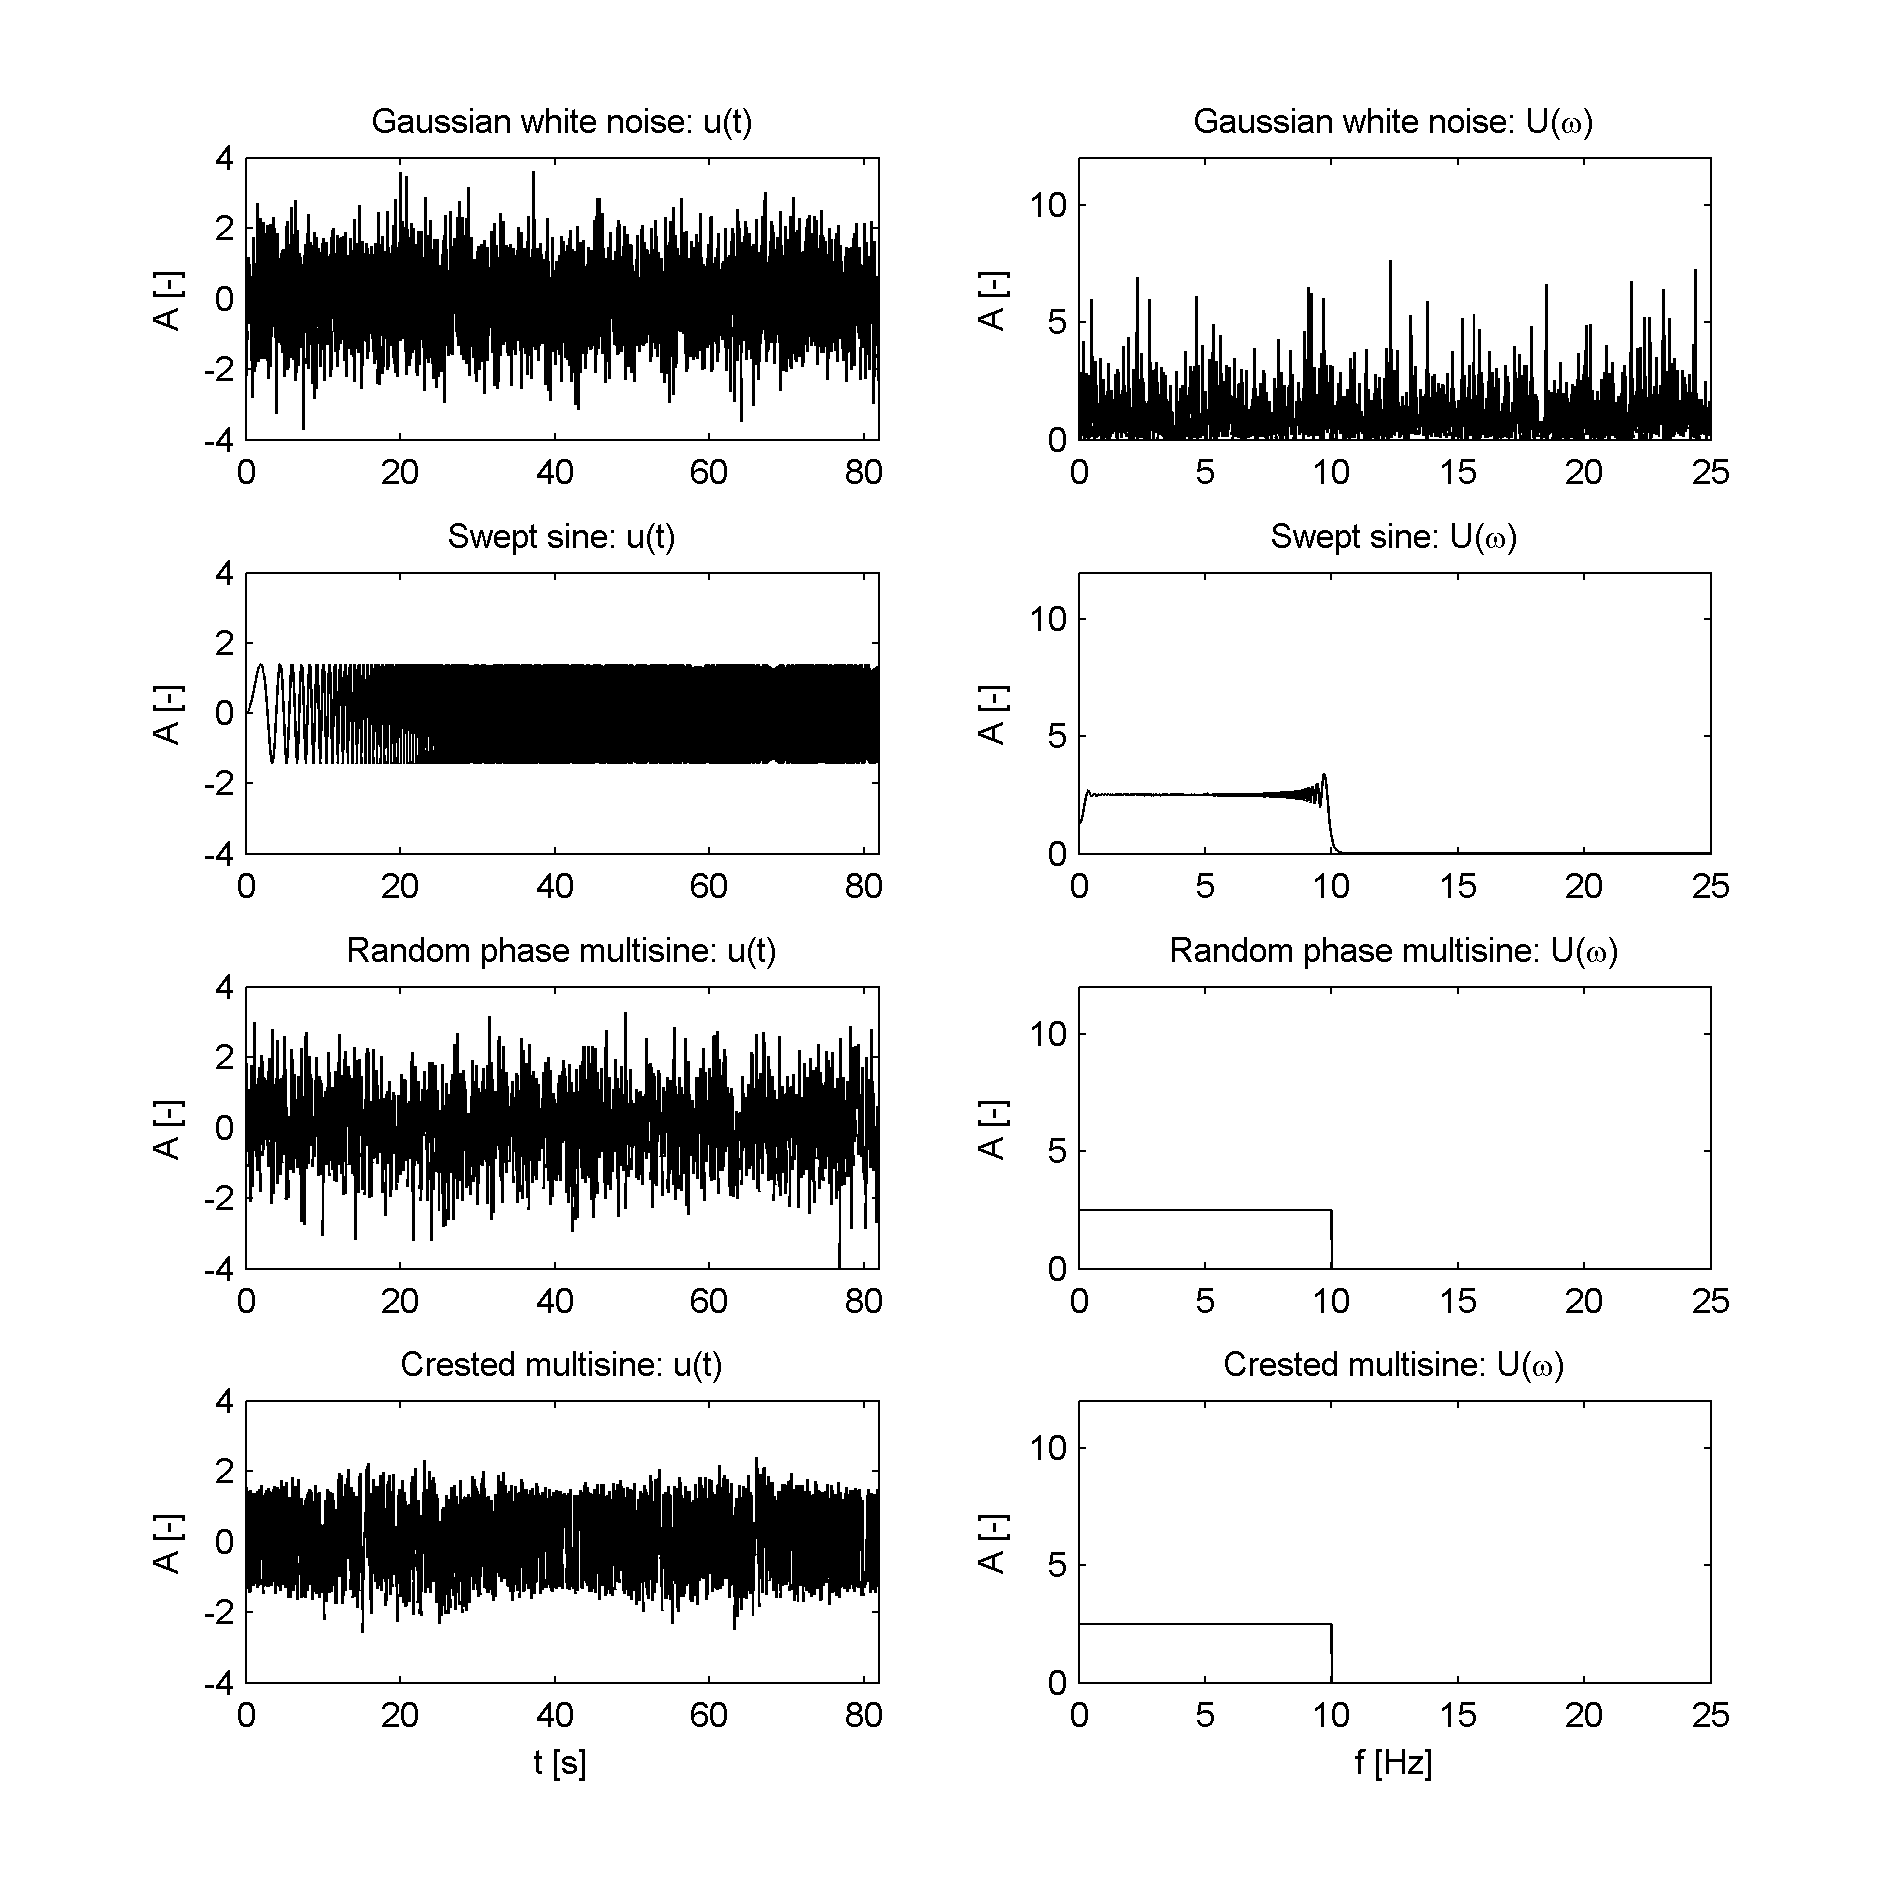
\includegraphics{images/u}
			\label{fig:u}
			\caption{4 different input signals: Gaussian white noise, swept sine, random phase multisine, crested random phase multisine}
		\end{figure}
\begin{table}
		\centering
		\begin{tabular}{lrrrr}
		\toprule
																			& White noise & Swept sine & Multisine & Crested  \\
		\midrule
		Mean ($\mu_u$):					& 0 & 0 & 0 & 0 \\
		Correlation ($R_{uu}$):	& 1 & 1 & 1 & 1 \\
		Spectral density ($S_{uu}):$ 										& 1.0145 &   2.4912  &  2.5000  &  2.5000 \\
		Crest factor ($C$): 						& 3.6129   & 1.4026  &  3.2857   & 2.3943 \\
		Predictable: 								& no & yes & no & no \\
		\bottomrule
		\end{tabular}
		\label{table:u}
		\caption{Comparison of various input signals. Notice that the spectral density is defined as the average spectral density over the desired frequency band.}
\end{table}
\subsection{Results}
The multisine offers the best results, but is predicatable, therefore the crested multisine is advised when identifying  the human controller.
\section{Frequency averaging}
Frequency averaging is used to reduce the influence of noise in the frequency domain at the cost of a decreased frequency resolution. There are 2 commonly used methods for frequency averaging; frequency block averaging and averaging over neighbouring frequencies. Yet to be described in more detail. 
\section{SISO identification}
Suppose we measure both the steering torque $T_\delta$ and roll angle $\phi$. This can be modelled as a simple open loop, single input, single output system. This corresponding block diagram is shown below:
%\begin{figure}{h!}
	\begin{center}
		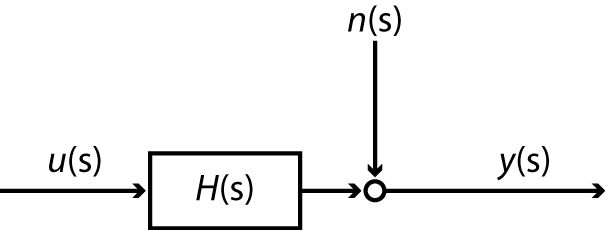
\includegraphics{images/SISOblock}
		%		\caption{Blockdiagram of the SISO model}
		\label{fig:SISOblock}
	\end{center}
	Where $u = u(s)$ represents the steering torque $T_\delta$ input, $\hat{y}= y(s)$ represents the measured output and $n= n(s)$ represents the measurement noise. 
\subsection{Simulation}
The linearized benchmark equations are used for the simulation. A forward velocity of 5 m/s is chosen, which results in stable dynamic behavior of the bicycle. The transferfunction from steering torque $T_\delta$ to roll angle $\phi$ is derived and yields (in zero-pole-gain form):
\begin{align}
H =   \frac{  -0.12262 (s+58.91) (s+13.77)  }{ (s+0.35) (s+14.27) (s^2 + 1.594s + 19.53) } 
\end{align}
This model will be used to simulate the bicycle response. Later on we will assume the system to be unknown and use system identification and parameter estimation techniques to estimate the  transfer function. Naturally the following question arises; ''why bother estimating a system that is already known?'. De answer to this this question is that we are actually interested in the quality of the identification procedures. The quality of the estimated fit can easily be checked by comparing it with the true system.

A simulation is set up, using the following measurement parameters:
			\begin{center}
				\begin{tabular}{lccc}
				\toprule
				description & symbol & value & units  \\
				\midrule
					Measurement time	 &	T    					& $100	$							& [s] 		\\
					Sample frequency	 &		$f_s$   			& $50		$							& [Hz] 	\\
					Sample period				 &	$\Delta T$ & $1/f_s$ 							& [s] 		\\
					Number of samples &		$N$    			& $T/\Delta T	$			& [-]			\\
					Input bandwidth & $f_{bw}$ & $2$                   & [Hz] \\
					\bottomrule
				\end{tabular}
			\end{center}
The input signal $u$ is designed as an crested multisine, which is described in the previous chapter. The maximum torque is set to 0.6 Nm. The standard deviation of the noise is set to 0.01 rad.
Next the simulation is started resulting in the measured output $y(t)$. The input and output are then converted to the frequency domain, spectral densities are calculated and finally some frequency averaging (not discussed) is applied in order to reduce the noise.
\subsection{System identification}
Next we will use the simulated dataset to derive the transfer function of the system. Starting from the block diagram shown in figure \ref{fig:SISOblock} we can derive the following equation:
\begin{align}
		Hu & = y-n 
\end{align}
Unfortuneatly we don't know the the noise $n$, which makes solving for $H$ impossible. However we can find a linear estimation of the system by seeking a solution under the image of $u$. This is achieved by projecting $u$ onto the left side of the equations. Assuming the noise is uncorrelated with the input (they are 2  independent signals), the linear estimated transferfunction $\hat{H}$ can be derived:
\begin{align}
		u^\ast Hu & = u^\ast (y-n) \nonumber \\
		H 					& = \frac{u^\ast (y-n)}{u^\ast u}  \nonumber \\
		\hat{H}	& = \frac{u^\ast y}{u^\ast u} \nonumber \\
		\hat{H} 	& = \frac{S_{uy}}{S_{uu}}
		\label{eq:SISOH}
\end{align}
Here $S_{uy}$ represent the cross spectral density of the input/output and $S_{uu}$ represents the auto spectral density of the input. The resulting tranferfunction is shown as a bode function in figure \ref{fig:SISObode}. The gain of the transfer function decreases as the frequency increases, resulting in a poorer signal to noise ratio at higher frequencies. Also notice that the input signal contains frequency content ranging from 0 to 2 Hz. Above 2 Hz the response is dominated completly by the noise. The coherence represents the linear estimation quality of the transfer function. As expected, the coherence drops dramatically above 2 Hz.
	\begin{figure}
		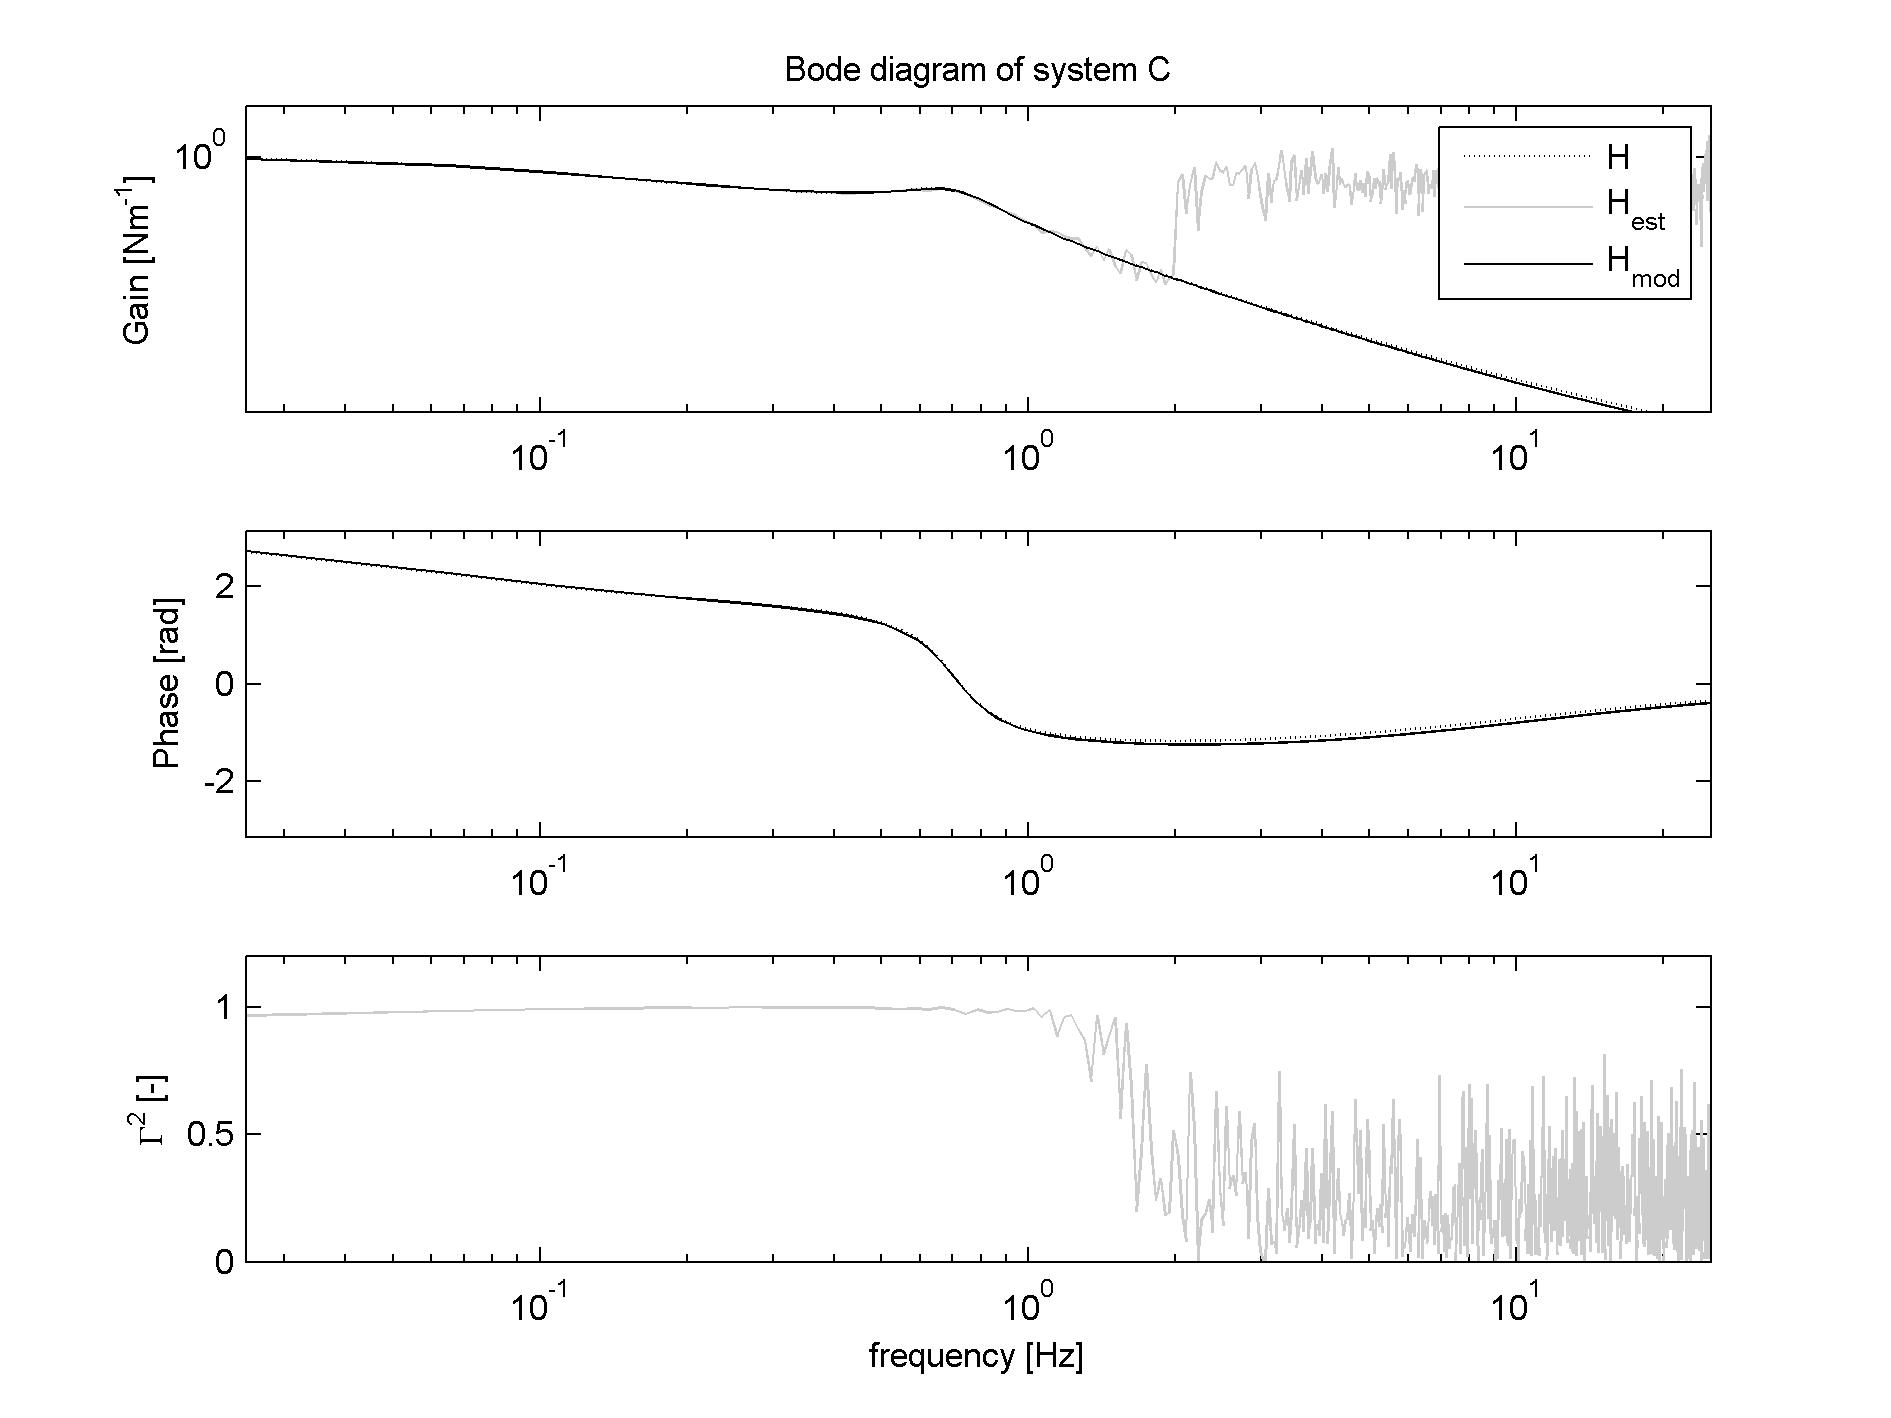
\includegraphics{images/SISObode}
		\caption{Bode diagram of the true ($H$), estimated ($H_{est}$) and parametric ($H_{mod}$) transfer function.}
				\label{fig:SISObode}
	\end{figure}
\subsection{Parameter estimation}
The estimated tranferfunction can then be used to determining the actual parameters of the transferfunction. We assume a solution of the following form:
	\begin{align}
		H_{\textrm{mod}}(s,x_i) = \frac{ x_1 (s+x_2) (s+x_3)  }{ (s+x_4) (s+x_5) (s^2 + x_6s + x_7) } 
	\end{align}
The error function is chosen to be:
		\begin{equation}
		e_s = \sqrt{\frac{1}{2\pi\omega_s}}\gamma(\omega_s)\left|\ln \hat{H}(\omega_s)-\ln H_{mod}(\omega_s,x_i)\right|
		\end{equation}
Here the $1\omega$ term acts as a weightening function, which puts more weight on lower frequencies. The $\ln$ function puts more weight on errors at lower magnitudes. This error definition is commonly used when fitting in the frequency domain. The reason to use these special weightnings is to counteract the logarithmic scale of a bode magnitude plot.
The criterium thus becomes:
		\begin{equation}
		J = \frac{1}{2}\sum_{s} e_s^2
		\end{equation}	
The Matlab \mcode{lsqnonlin} algorithm is used for the optimization. The resulting parameters together with the true parameters are shown in table \ref{table:SISOparms}.
\begin{table}
\centering
		\begin{tabular}{cccc}
		\toprule
		$x_i$ & True & Estimated & $\sigma_{\mu_{x_i}}$ \\
		\midrule
		$x_1$&   -0.1112  	& -0.1226  	&  0.1241\\
		$x_2$&	58.0972   	&58.9100  	& 89.8280\\
    $x_3$&	7.3382   		&13.7700  	& 35.0404\\
    $x_4$&	0.3715   		& 0.3500  		&  0.0295\\
    $x_5$&	6.6603   		&14.2700  	& 29.0601\\
    $x_6$&	1.5845    	&1.5940  		&  0.1576\\
		$x_7$&	19.7927  	&19.5300 		&   0.6974\\
		\bottomrule
 		\end{tabular}
		\caption{Comparison of the estimated parameters with the true parameters. $\sigma_{\mu_{x_i}}$ represents the standard deviation of the mean.}
		\label{table:SISOparms}
\end{table}
The quality of the resulting parameters is varying. Some parameters ar more difficult to fit than others. When we look at the true system (equation \ref{eq:SISOH}), we observe a near zero/pole cancelation of the 3th and 5th parameter, which renders them practically unobservable. This makes these parameters very hard to  fit, which results in a huge uncertainty in the estimation these 2 corresponding parameters. The low quality fit of parameter 2 is unknown at this point. Possibly the optimization algorithm got stuck on a global minimum. The resulting fit (shown in figure \ref{fig:SISObode} seems pretty good however.
\section{MIMO identification}
Next we are interested in estimating the complete bicycle equations. The system has two inputs; rolling torque $T_\phi$ and steering torque $T_\delta$. The following outputs are measured; roll angle $\phi$ and steerangle $\delta$. Since the system has multiple inputs and multiple outputs we have to apply MIMO system identification techniques. The corresponding block diagram is shown below:
	\begin{center}
		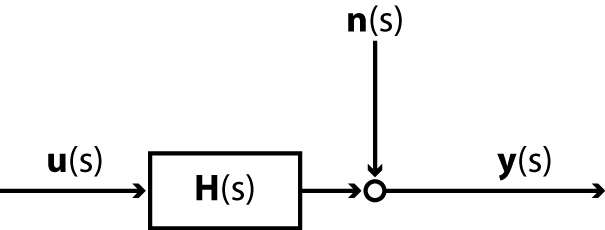
\includegraphics{images/MIMOblock}
		%		\caption{Blockdiagram of the SISO model}
		\label{fig:MIMOblock}
	\end{center}
Where $\mathbf{u} = \mathbf{u}(s)$ represents the input vector, $\mathbf{y}= \mathbf{y}(s)$ represents the measured output vector and $\mathbf{n} = \mathbf{n}(s)$ represents the measurement noise vector. The block diagram looks pretty similar to the SISO case, except here the scalar function are replaced by vectors and matrices.
\subsection{Simulation}
Again the linearized benchmark equations are used for the simulation. A forward velocity of 5 m/s is chosen, which results in stable dynamic behavior of the bicycle. The governing input/output relationship is shown below in state space form:
	\begin{align}
		\mathbf{\dot{x}} & = \mathbf{A}\mathbf{x} + \mathbf{B}\mathbf{u} \nonumber \\
		\mathbf{y} & = \mathbf{C}\mathbf{x} 
	\end{align}
Where;
	\begin{align}
	{\scriptstyle
			\mathbf{A} =   \left[\begin{array}{cccc} 
									$0$ & $0$ & $1$ & $0$ \\
									$0$ & $0$ & $0$ & $1$ \\
									$9.470$ & $-22.758$ & $-0.520$ & $-1.638$ \\
									$12.400$ & $-19.499$ & $18.089$ & $-15.694$   
			\end{array}\right]   \nonumber \ \ , \
			\mathbf{B} = \left[\begin{array}{cc}
									 $0$ & $0$ \\
									$0$ & $0$ \\
									$0.016$ & $-0.123$ \\
									$-0.123$ & $4.265$ 
			\end{array}\right] \nonumber \ \ , \ 
			\mathbf{C} = \left[\begin{array}{cccc}
									$1$ & $0$ & $0$ & $0$ \\
									$0$ & $1$ & $0$ & $0$
			\end{array}\right]  \nonumber
	}
	\end{align}
A simulation is set up, using the same measurement parameters as for the SISO case (see table: \ref{table:SISOparms}. The input signal $\mathbf{u}$ is designed as an crested multisine which will be explained later on in more detail. The maximum steering torque is set to 0.6 Nm and the maximum roll torque is set to 10 Nm. The standard deviation of the noise for all measured outputs is set to 0.01 rad. The simulation is run twice, with different input vectors. 
\subsection{MIMO system identification}
Next we will use the simulated dataset to derive the transfer function of the system. Starting from the block diagram shown in figure \ref{fig:MIMOblock} we can derive the following equation:
\begin{align}
		\mathbf{H}\mathbf{u} & = \mathbf{y}-\mathbf{n} 
\end{align}
Unfortuneatly this system is not solvable, since we can't invert the inputvector $\mathbf{u}$. Therefore we need additional measurements. A nice choice of input would be the following:
\begin{align}
		\mathbf{U}(s) = \left[\begin{array}{cc}
									A_\phi &  A_\phi \\
									A_\delta & -A_\delta \\
			\end{array}\right] u(s)
\end{align}
Where $A_\phi=5$ and $A_\delta=0.6$ are amplification gains which are found by trial and error. Similar as in the SISO case we will seek a solution in the image of $\mathbf{U}$. Here only need to be a little bit more carefull, since the multiplication of vectors and matrices is generally non-communicative.
\begin{align}
		\mathbf{H}\mathbf{U} & = \mathbf{Y}-\mathbf{N}  \nonumber \\
		\mathbf{U}^\ast\mathbf{H}^\ast & = \mathbf{Y}^\ast-\mathbf{N} ^\ast \nonumber \\
			\mathbf{U}\mathbf{U}^\ast\mathbf{H}^\ast & = 	\mathbf{U}\left(\mathbf{Y}^*-\mathbf{N} ^\ast\right) \nonumber \\
			\mathbf{H}^\ast & = 	\left(\mathbf{U}\mathbf{U}^\ast\right)^{-1}\mathbf{U}\left(\mathbf{Y}^\ast-\mathbf{N} ^\ast\right) \nonumber \\
						\mathbf{H} & = 	\left(\mathbf{Y}-\mathbf{N}\right)\mathbf{U}^\ast\left(\mathbf{U}\mathbf{U}^\ast\right)^{-1} 
\end{align}
Next we define the estimated transferfunction $\hat{\mathbf{H}}$ to be the transferfunction that linearly correlates the input/output data, assuming that the input is independent of the noise ($\mathbf{N}\mathbf{U}^\ast \approx \mathbf{0}$). 
\begin{align}
						\hat{\mathbf{H}} 	= & \mathbf{Y}\mathbf{U}^\ast\left(\mathbf{U}\mathbf{U}^\ast\right)^{-1} \nonumber \\
																			= & \mathbf{S}_{yu}\mathbf{S}_{uu}^{-1}
		\label{eq:MIMOH}
\end{align}
Here $S_{uy}$ represent the cross spectral density of the input/output and $S_{uu}$ represents the auto spectral density of the input. The resulting tranferfunction is shown as a bode function in figure \ref{fig:SISObode}. The gain of the transfer function decreases as the frequency increases, resulting in a poorer signal to noise ratio at higher frequencies. Also notice that the input signal contains frequency content ranging from 0 to 2 Hz. Above 2 Hz the response is dominated completly by the noise. The coherence represents the linear estimation quality of the transfer function. As expected, the coherence drops dramatically above 2 Hz.
	\begin{figure}
		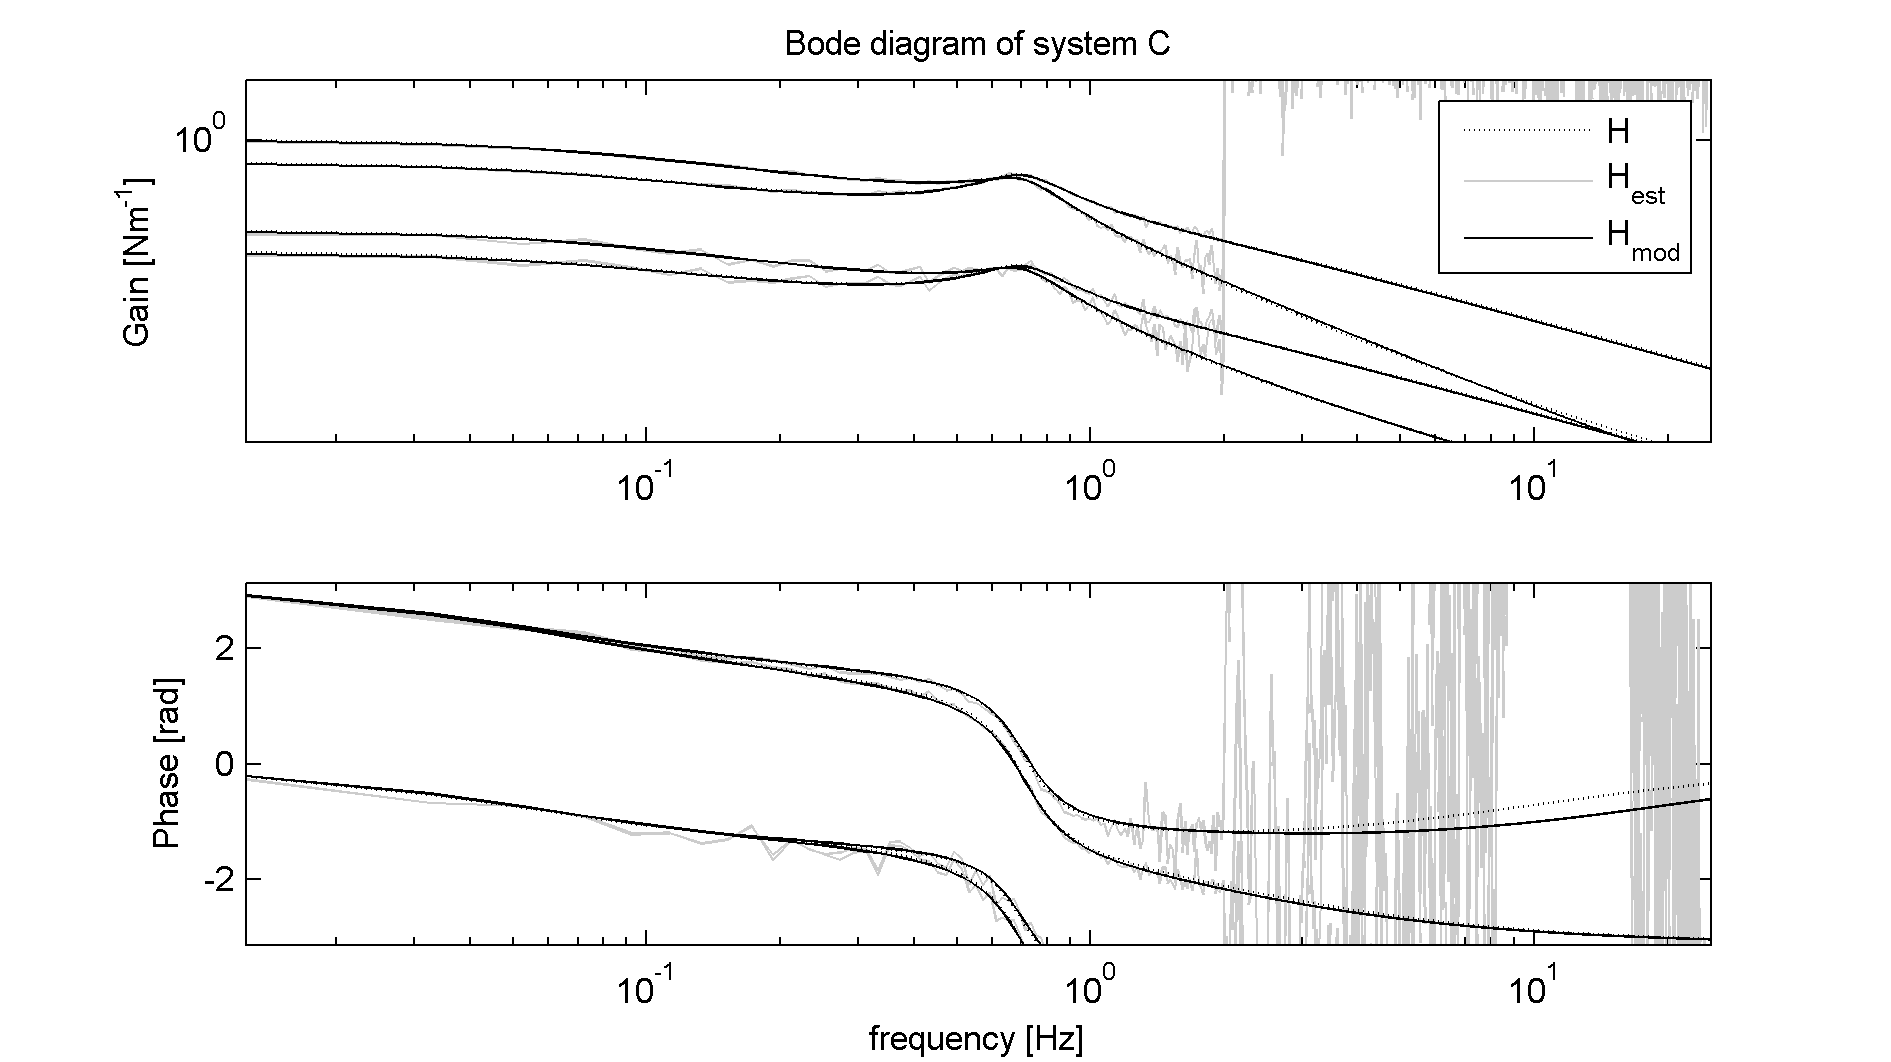
\includegraphics{images/MIMObode}
		\caption{Bode diagram of the true ($H$), estimated ($H_{est}$) and parametric ($H_{mod}$) transfer function.}
				\label{fig:MIMObode}
	\end{figure}
	\subsection{MIMO parameter estimation}
	Yet to be done.
 
\chapter{Rider identification}
Time domain identification using ARX models appears to be a promising way to estimate the rider transferfunction. Dr. Ron Hess is currently experimenting with these models and has already derived some nice results. Also, the choice of input signal is way more flexible then typical frequency domain estimation signals. For example; step inputs, and impulses seem to work really wel. Jason has constructed a rope with force sensor which could be used to apply known perturbations to the bicycle. I'm hoping to find ou more on time domain identification and parameter estimation next week. Another method would be the output error method, which used parameter optimization techniques to fit a parametric model onto the measured output data.
\section{ARX model}
Yet to be described. Ask Dr. Hess.
\section{Output Error model}
Output Error models offer an simple way to validate the measured output (steering torque in this case). Let's assume that the rider only excerts steering torque and knows the configuration of the bicycle $\mathbf{q}$. The rol angle $\phi_c$ is considered the control objective and no external excitation is present. In this case, the steering torque is expected to be some function of the desired roll angle and configuration of the bicycle:
		\begin{align}
		T_\delta = {K}(\mathbf{q},\phi_c)
		\end{align}
At this point the function could be of any form, it could be linear/non-linear,  may include differentials/integrals, could be discontinues/continues, include time delays, etc. %A block form representation is given in the figure below.
%\begin{figure}[ht]
\centering %

% We need layers to draw the block diagram
\pgfdeclarelayer{background}
\pgfdeclarelayer{foreground}
\pgfsetlayers{background,main,foreground}


\tikzstyle{block} = [draw,rectangle,thick,minimum height=2em,minimum width=2em]
\tikzstyle{bigblock} = [draw,rectangle,thick,minimum height=2em,minimum width=3em]
\tikzstyle{sum} = [draw,circle,inner sep=0mm,minimum size=2mm]
\tikzstyle{connector} = [->,thick]
\tikzstyle{line} = [thick]	

\tikzstyle{branch} = [circle,inner sep=0pt,minimum size=1mm,fill=black,draw=black]
\tikzstyle{guide} = []

\def \myneq {\skew{-2}\not =} % \neq alone skews the dash

\begin{tikzpicture}[scale=1, auto, >=stealth']

    %  Loop function
    \node[coordinate]												(input) 		{};
		\node[coordinate,right of=input]		(sumphi)	{};
		\node[block,right of =sumphi] 			(K) 					{${K}$};
		\node[coordinate,right of=K]				(Tdelta)		{$T_\delta$};
		\node[block,right of =Tdelta]				(H) 					{$\mathbf{H}$};
		\node[coordinate,right of =H]				(phi) 				{};
    \node[coordinate, right of=phi]			(output) 	{};
		
		% Feedback paths
		\node[coordinate,below of=H]			(fbH)				{};
		\node[coordinate,below of=K]			(fbK)				{};
		
		% Draw connectors
		\draw[connector] (input) -- node {$\phi_c$} (K);
		\draw[connector] (K) -- node {$T_\delta$} (H);
		\draw[connector] (H) -- node {$\phi$} (output);
		
		\draw[line] (H) -- (fbH)  -- node {$\mathbf{q}$}  (fbK);
		\draw[connector] (fbK) -- (K);
		
		
			
		%% Feedback nodes
		%\path (H.center)+(-0.75em,-0.65em) node (Hdelta) {}; 	\node[coordinate,below of=Hdelta](fbHdelta){};
		%\path (H.center)+(-0.25em,-0.65em) node (Hphid) {};		\node[coordinate,below of=Hphid](fbHphid) {};
		%\path (H.center)+( 0.25em,-0.65em) node (Hphi) {};			\node[coordinate,below of=Hphi](fbHphi){};
		%\path (H.center)+( 0.75em,-0.65em) node (Hpsi) {};			\node[coordinate,below of=Hpsi](fbHpsi){};
		%\path (y.center)+( 0.00em,-0.65em) node (Hy) {};	  	\node[coordinate,below of=Hy](fbHy){};
%
		%% Multiple loop feedback
		%\draw [line] (Hdelta) -- 	node {} ([yshift=-0em] fbHdelta) ;
		%\draw [line] (Hphid) -- 		node {} ([yshift=-1em] fbHphid) ;
		%\draw [line] (Hphi) -- 			node {} ([yshift=-2em] fbHphi) ;
		%\draw [line] (Hpsi) -- 			node {} ([yshift=-3em] fbHpsi) ;
		%\draw [line] (y) -- 						node {} ([yshift=-4em] fbHy) ;
		%
		%\draw [connector] ([yshift=-0em] fbHdelta) [line]  -| node {$\delta$} (sumdelta) 			;
		%\draw [connector] ([yshift=-1em] fbHphid) [line]  -|  node {$\dot{\phi}$} (sumphid)	;
		%\draw [connector] ([yshift=-2em] fbHphi) [line]  -| 	node {$\phi$} (sumphi) 								;
		%\draw [connector] ([yshift=-3em] fbHpsi) [line]  -| 	node {$\psi$} (sumpsi) 						;
		%\draw [connector] ([yshift=-4em] fbHy) [line]  -| 	node {$y$} (sumy)										;
		%
		%\draw (sumdelta) node[below left] {$\scriptstyle-$} ;
		%\draw (sumphid) node[below left] {$\scriptstyle-$} ;
		%\draw (sumphi) node[below left] {$\scriptstyle-$} ;
		%\draw (sumpsi) node[below left] {$\scriptstyle-$} ;
		%\draw (sumy) node[below left] {$\scriptstyle-$} ;

    %\begin{pgfonlayer}{background}
        %% Compute a few helper coordinates
				%% RIder
				 %\path (Gnm.south east)+(+1em,-5.7em) node (b) {};
        %\path (Ky.north west)+(-0.5em,2em) node (a) {};
        %\path[fill=black!00,rounded corners=0.5em, draw=black!50, dashed]
						%(b) rectangle (a) node[below right, color = black!50] {Rider};
        %% Innerloop
				%\path (Gnm.south east)+(+0.5em,-3.7em) node (b) {};
				%\path (Kphi.north west)+(-0.5em,1.5em) node (a) {};
        %\path[fill=black!00,rounded corners=0.5em, draw=black!50, dashed]
						%(b) rectangle (a) node[below right, color = black!50] {Inner loop};
				%% Bike
				%\path (H.south east)+(+0.5em,-5.7em) node (b) {};
				%\path (H.north west)+(-0.5em,2em) node (a) {};
        %\path[fill=black!00,rounded corners=0.5em, draw=black!50, dashed]
						%(b) rectangle (a) node[below right, color = black!50] {Bike};					
    %\end{pgfonlayer}
    \end{tikzpicture}
\caption{Block diagram for general control models concerning roll angle control, without external excitation.}

\label{fig:hessblock}

\end{figure}
\subsection{Parametric models}
Next the human controller is modelled as a parametric model. This is achieved by assuming a solution of any form, which can be optimized by changing the values of the parameter vector $\boldsymbol{\theta}$. The parameterized model is given by:
		\begin{align}
		\hat{T}_\delta = \hat{K}(\boldsymbol{\theta},\mathbf{q},\phi_c)
		\end{align}
\subsection{Output error model}
The output error model is used to compare the measured data with the model simulation data. The model returns the error between the outputs of the two systems. In order to apply this method, one should measure the steering torque and bicycle configuration. The desired roll angle is determined to be zero, which corresponds to balancing the bike in an upright position. The measured configuration $\mathbf{q}$ is then inserted in the parametric model, which outputs steering torque $\hat{T}_\delta$. The error $e(t)$ is defined as the difference between the measured and modelled simulation data. The resulting model is shown in the block diagram (ref?). Finally, the following well known criterium function is set up to determine the quality of the fit:
    \begin{figure}[ht]
\centering %

% We need layers to draw the block diagram
\pgfdeclarelayer{background}
\pgfdeclarelayer{foreground}
\pgfsetlayers{background,main,foreground}


\tikzstyle{block} = [draw,rectangle,thick,minimum height=2em,minimum width=2em]
\tikzstyle{bigblock} = [draw,rectangle,thick,minimum height=2em,minimum width=3em]
\tikzstyle{sum} = [draw,circle,inner sep=0mm,minimum size=2mm]
\tikzstyle{connector} = [->,thick]
\tikzstyle{line} = [thick]	

\tikzstyle{branch} = [circle,inner sep=0pt,minimum size=1mm,fill=black,draw=black]
\tikzstyle{guide} = []

\def \myneq {\skew{-2}\not =} % \neq alone skews the dash

\begin{tikzpicture}[scale=1, auto, >=stealth']

    %  Loop function
    \node[coordinate]												(input) 		{};
		\node[coordinate,right of=input]		(sumphi)	{};
		\node[bigblock,right of =sumphi] 	(K) 					{$K$};
		\node[coordinate,right of=K]				(tmp1)		{};
			\node[coordinate,right of=tmp1]				(Tdelta)		{};

		\node[coordinate,right of =Tdelta]				(output1) {$T_\delta$};
		
		% Feedback paths
		\node[block,below of = Tdelta]			(H)					{$\mathbf{H}$};

		\node[coordinate,below of=K]			(q)					{};
		\node[sum,right of=H]									(sume)		{};
		\node[coordinate,right of=sume]	(OE)				{};

		
		% Parametric
		\node[bigblock, below of=q]				(K2)					{$\hat{K}$};
		\node[coordinate,right of=K2]				(tmp2)		{};
		\node[coordinate,right of=tmp2]					(Tdelta2)		{};
		\node[coordinate,right of =Tdelta2]	(output2) 	{$\hat{T}_\delta$};


		% Draw connectors
		\draw[connector] (input) -- node {$\phi_c$} (K);
		\draw[connector] (sumphi) |- node {} (K2);
		\draw[line] (K) -- node {$T_\delta$} (output1);
		\draw[connector] (output1) -- node {} (sume);

		\draw[connector] (Tdelta) -- node {} (H);
		\draw[line] (H)-- node {$\mathbf{q}$} (q);
		\draw[connector] (q)-- node {} (K);
		\draw[connector] (q)-- node {} (K2);
		\draw[line] (K2) -- node[below]  {$\hat{T}_\delta$} (output2);
		\draw[connector] (output2) -- node {} (sume);
		\draw[connector] (sume) -- node {$e$} (OE);


    \end{tikzpicture}
\caption{Output error model for the rider estimation}

\label{fig:outputerror}

\end{figure}
		\begin{align}
		J = \frac{1}{2}\sum_i\left(\tilde{T}_{\delta,i} - \hat{T}_{\delta,i} \right)^2
		\end{align}
This criterium can be used to compare different models for the human controllers. A value of zero indicates a perfect fit, whereas higher values of $J$ indicate larger errors. The criterium function can also be used to optimize the model parameter vector.
 
\chapter{Bicycle simulator}
As a simple experiment, a computer bicycle simulator is created. The user control the velocity and steering torque using a controller and receives visual feedback of the 3D bicycle visualisation, roll angle indicator, roll velocity indicator, applied torque indicator and velocity indicator. The work described is purelly experimental and is not yet ready for scientific purposes. 
\section{Linear simulation}
First, the linear bicycle equations for the benchmark bicycle are implemented within the bicycle simulator. 
		\begin{align} 
		\mathbf{M}\ddot{\mathbf{q}} + v\mathbf{C}_1\dot{\mathbf{q} } + \left[g\mathbf{K}_0 + v^2\mathbf{K}_2\right]\mathbf{q} = \mathbf{f} \ ,
		\end{align}
where; $\mathbf{q} = \left[\phi , \ \delta \right]^T$ and $\mathbf{f} = \left[ T_\phi , \ T_\delta \right]^T$. As said the user input consists of: velocity; $v$ [m/s] and steering torque; $T_{\delta}$ [Nm]. The lean action is omitted, but would be interesting to include later on in the simulation.
\subsection{Results}
			\begin{itemize}
			\item Control generally seems to be done intermittently. 
			\item Dynamic behavior of the bicycle changes as function of the forward velocity; $v$.
			\item Capsize instability easy to control. 
			\item At low velocity the weave mode becomes instable and becomes very hard to control.
			\item Linear equations only valid for small angles.
			\item Adding visual cue about roll rate makes control below the weave speed a lot easier.
			\end{itemize}
\section{Non-linear simulation}
Next the non-linear equations (provided by Luke) where inserted into the simulator. After overcoming technical diffuculties with the C-compiling of the non-linear equations (error: expressions to complicated), the non-linear equations where easy to implement. The velocity in Luke's equations is defined a little different than the linearized equations. In the non-linear equations the velocity is defined at the frontwheel contact point, while in the linear equations the velocity is defined in the rearwheel contact point. This results in a somewhat overestimated velocity, because the difference traveled by the front wheel contact point is expected to be larger than the rear or CoM contact point. In the next paragraph some interesting results are pointed out.
\subsection{Results}
			\begin{itemize}
			\item A strong coupling between roll angle and velocity exists (maybe caused by wrong velocity definition).
			\item Unexpected stable weave like oscilations occur below the weave velocity. 
			\item Controlling unstable weave mode appears to be similar as during the linear equations.
			\end{itemize}
\section{Future work}
The following items would be interesting to implement:
			\begin{itemize}
			\item Definition: velocity of the rearwheel contact point.
			\item Energy tracking to check for energy conservation.
			\item Add force feedback to include proprioceptive conrol loop.
			\end{itemize}
 
\include{control} 
\include{other} 
\section{Multiple loop rider model}
In this chapter the rider model presented by Dr. Hess will be analyzed. The block diagram of the rider/bicycle model is shown in figure \ref{fig:hessblock}. The rider is modelled as an multi loop feedback controller. The gains denoted by $K$ are the feedback gains of the human controller. These gains are actually yet to be identified, but estimates are provided by Dr. Hess. Block $G_{nm}$ represents the neuromuscular dynamics and block $\mathbf{H}$ contains the bicycle dynamics. 
\begin{figure}[ht]
\centering %

% We need layers to draw the block diagram
\pgfdeclarelayer{background}
\pgfdeclarelayer{foreground}
\pgfsetlayers{background,main,foreground}


\tikzstyle{block} = [draw,rectangle,thick,minimum height=2em,minimum width=2em]
\tikzstyle{bigblock} = [draw,rectangle,thick,minimum height=2em,minimum width=3em]
\tikzstyle{sum} = [draw,circle,inner sep=0mm,minimum size=2mm]
\tikzstyle{connector} = [->,thick]
\tikzstyle{line} = [thick]

\tikzstyle{branch} = [circle,inner sep=0pt,minimum size=1mm,fill=black,draw=black]
\tikzstyle{guide} = []
\tikzstyle{input} = [coordinate]
\tikzstyle{output} = [coordinate]

\renewcommand{\vec}[1]{\ensuremath{\boldsymbol{#1}}} % bold vectors
\def \myneq {\skew{-2}\not =} % \neq alone skews the dash

\def\edgedist{0.1}

\begin{tikzpicture}[scale=1, auto, >=stealth']
    %\small
    \node [input, name=input] {};
				\node[sum,right of=input] (sumy){};
		\node[block,right of =sumy] (Ky) {$K_y$};
				\node[sum,right of=Ky] (sumpsi){};
		\node[block,right of =sumpsi] (Kpsi) {$K_\psi$};
				\node[sum,right of=Kpsi] (sumphi){};
		\node[block,right of =sumphi] (Kphi) {$K_\phi$};
				\node[sum,right of=Kphi] (sumphid){};
		\node[block,right of =sumphid] (Kphid) {$K_{\dot{\phi}}$};
				\node[sum,right of=Kphid] (sumdelta){};
		\node[block,right of =sumdelta] (Kdelta) {$K_\delta$};
				\node[right of = Kdelta,coordinate](c) {};
		\node[block,right of =c] (Gnm) {$G_{nm}$};
				\node[right of = Gnm,coordinate](u) {};
		\node[bigblock,right of =u](H) {$\mathbf{H}$};
				\node[branch,right of = H](y) {};
    \node [output, right of=y ](output) {};
		% Feedback nodes
		\node[coordinate,above of=H] (Tphi) {};

				% Disturbance
		\draw [connector] ([yshift=2em] Tphi)  -- node[above right] {${T_\phi}$} (H);
		
		% Draw connectors
		\draw [connector] (input) -- node {$y_c$} (sumy);
				\draw [connector] (sumy) -- node {} (Ky);
		\draw [connector] (Ky) -- node {} (sumpsi);
				\draw [connector] (sumpsi) -- node {} (Kpsi);
		\draw [connector] (Kpsi) -- node {} (sumphi);
				\draw [connector] (sumphi) -- node {} (Kphi);
		\draw [connector] (Kphi) -- node {} (sumphid);
				\draw [connector] (sumphid) -- node {} (Kphid);
		\draw [connector] (Kphid) -- node {} (sumdelta);
						\draw [connector] (sumdelta) -- node {} (Kdelta);
		\draw [connector] (Kdelta) -- node {} (Gnm);
		\draw [connector] (Gnm) -- node {$T_\delta$} (H);
		\draw [connector] (H) -- node {${y}$} (output);
			
		% Feedback nodes
		\path (H.center)+(-0.75em,-0.65em) node (Hdelta) {}; 	\node[coordinate,below of=Hdelta](fbHdelta){};
		\path (H.center)+(-0.25em,-0.65em) node (Hphid) {};		\node[coordinate,below of=Hphid](fbHphid) {};
		\path (H.center)+( 0.25em,-0.65em) node (Hphi) {};			\node[coordinate,below of=Hphi](fbHphi){};
		\path (H.center)+( 0.75em,-0.65em) node (Hpsi) {};			\node[coordinate,below of=Hpsi](fbHpsi){};
		\path (y.center)+( 0.00em,-0.65em) node (Hy) {};	  	\node[coordinate,below of=Hy](fbHy){};

		% Multiple loop feedback
		\draw [line] (Hdelta) -- 	node {} ([yshift=-0em] fbHdelta) ;
		\draw [line] (Hphid) -- 		node {} ([yshift=-1em] fbHphid) ;
		\draw [line] (Hphi) -- 			node {} ([yshift=-2em] fbHphi) ;
		\draw [line] (Hpsi) -- 			node {} ([yshift=-3em] fbHpsi) ;
		\draw [line] (y) -- 						node {} ([yshift=-4em] fbHy) ;
		
		\draw [connector] ([yshift=-0em] fbHdelta) [line]  -| node {$\delta$} (sumdelta) 			;
		\draw [connector] ([yshift=-1em] fbHphid) [line]  -|  node {$\dot{\phi}$} (sumphid)	;
		\draw [connector] ([yshift=-2em] fbHphi) [line]  -| 	node {$\phi$} (sumphi) 								;
		\draw [connector] ([yshift=-3em] fbHpsi) [line]  -| 	node {$\psi$} (sumpsi) 						;
		\draw [connector] ([yshift=-4em] fbHy) [line]  -| 	node {$y$} (sumy)										;
		
		\draw (sumdelta) node[below left] {$\scriptstyle-$} ;
		\draw (sumphid) node[below left] {$\scriptstyle-$} ;
		\draw (sumphi) node[below left] {$\scriptstyle-$} ;
		\draw (sumpsi) node[below left] {$\scriptstyle-$} ;
		\draw (sumy) node[below left] {$\scriptstyle-$} ;

    \begin{pgfonlayer}{background}
        % Compute a few helper coordinates
				% RIder
				 \path (Gnm.south east)+(+1em,-5.7em) node (b) {};
        \path (Ky.north west)+(-0.5em,2em) node (a) {};
        \path[fill=black!00,rounded corners=0.5em, draw=black!50, dashed]
						(b) rectangle (a) node[below right, color = black!50] {Rider};
        % Innerloop
				\path (Gnm.south east)+(+0.5em,-3.7em) node (b) {};
				\path (Kphi.north west)+(-0.5em,1.5em) node (a) {};
        \path[fill=black!00,rounded corners=0.5em, draw=black!50, dashed]
						(b) rectangle (a) node[below right, color = black!50] {Inner loop};
				% Bike
				\path (H.south east)+(+0.5em,-5.7em) node (b) {};
				\path (H.north west)+(-0.5em,2em) node (a) {};
        \path[fill=black!00,rounded corners=0.5em, draw=black!50, dashed]
						(b) rectangle (a) node[below right, color = black!50] {Bike};					
    \end{pgfonlayer}
    \end{tikzpicture}
\caption{Block diagram of the rider/bicycle model by Dr. Hess}

\label{fig:hessblock}

\end{figure}
The following expression in termse of the bicycle output and lateral objective displacement ($y_c$) can be derived from this block diagram and yields:
\begin{align}
		T_\delta 	&= G_{nm}K_\delta(K_{\dot{\phi}}(K_\phi(K_\psi(K_y(y_c-y)-\psi)-\phi)-\dot{\phi})-\delta) \nonumber
\end{align}
The neuromuscular dynamics are modelled as:
\begin{align}
		G_{nm} = \frac{30^2}{s^2 +  2(0.707)30s  + 30^2}
\end{align}
The bicycle dynamics can be expressed as a set of transfer functions:
\begin{align}
		\left[\begin{array}{c} \phi \\  \delta \\ \dot{\phi} \\ \dot{\delta} \\ \end{array} \right] = 
				\left[\begin{array}{cc} H_{11}  & H_{12} \\ H_{21}  & H_{22} \\ H_{31}  & H_{32} \\ H_{41}  & H_{42} \\  \end{array}\right]
				\left[\begin{array}{c} T_\phi \\ T_\delta \\ \end{array}\right]
\end{align}
And the additional output variables can be expressed in terms of the state variables as:
\begin{align}
		\psi 	&= \frac{1}{s}\frac{v\delta + c\dot{\delta}}{w}\cos\lambda \  , \\
		y			&\approx \frac{1}{s}v\psi \  \ \textrm{, for small angles of $\psi$.} 
\end{align}
Now we have all the ingredients to derive the combined system transfer functions, but first we will analyze possible ways of exciting the rider/bicycle combination.
\subsection{Possible ways to excite the system}
From the block diagram we observe the following two inputs; target lateral displacement $y_c$ and external disturbance $T_\phi$.  This is not completely correct, since it is also potentially possible to apply an external steering torque $T_{\delta\textrm{,ext}}$.  In general, an arbitrary external force applied at position $x_r$($= x_r(q_s)$) can be projected onto the generalized coordinates according to: 
\begin{align}
		T_{s\textrm{,ext}}  = \frac{\partial x_r}{\partial q_s} f_r \ ,
\end{align}  
where the Einstein summation convention is used to indicate summation over repeated indices. This operation results into the generalized external forces $T_{s\textrm{,ext}}$, which can be easially added to the dynamic equations of the bicycle.
		Caution is warranted when choosing the disturbance force, because certain choices me change the linearized dynamic behavior of the system.  In particular; it is important to apply the force orthogonal to the forward velocity component of the bicycle in order to prevent forward acceleration/deceleration. This matters, because changing the velocity affects the dynamics equations of the bicycle which are linearized around a certain constant velocity. The forward velocity could easially be changed, since the system is marginally stable in its velocity (e.i. forward motion is a rigid body mode).
		To conclude this section; the system can be excited by changing the varying the lateral displacement $y_c$ and by perturbing the system using an external disturbance force $f_r$.
\subsection{Overview of excitation schemes}
In table \ref{table:excitationscheme} a overview of possible ways of excitating the system is given. There are 2 possible external inputs; force and lateral objective displacement, which result in 4  possible combinations of exciting the system. 
\begin{table}
		\centering
		\begin{tabular}{c c l}
				\toprule
				Case & Excitation  & Description \\
				\midrule
				\multirow{2}{*}{1}
						& $y_c= 0$ 			&  \multirow{2}{*}{No external excitation} \\
						& $f_r = 0$ 			  & \\	\hline
				\multirow{2}{*}{2}
						& $y_c = 0$ 		  & \multirow{2}{*}{Excitation through force disturbance} \\
						& $f_r\neq0$ 		  & \\	\hline
				\multirow{2}{*}{3}
						& $y_c \neq 0$  & \multirow{2}{*}{Excitation through lateral displacement disturbance} \\
						& $f_r = 0$ 			  & \\	\hline
					\multirow{2}{*}{4}
						& $y_c \neq 0$  & \multirow{2}{*}{Combined excitation} \\
						& $f_r   \neq 0$  & \\
				\bottomrule
		\end{tabular}
		\caption{Possible ways to excite the systen}
		\label{table:excitationscheme}
\end{table}
\subsection{A case 2 application: force perturbations using rope}
A case 2 application is given in this section, where the system will be exited using a rope with force senor. Here, the rope is mounted on the bicycle below the seat and is being pulled manually by the experimenter. The subject is wearing lateral eye caps to prevent foreseeing the disturbance and thus excluding feedforward control. 
		The bicycle could be mounted on a tred mill, which would allow for easy perturbation. However, the tredmill could affect the experiment, since the limited road surface and danger of falling of could affect the riding style. Another possibility would be to ride the bicycle along a long straight line and perturb it with the rope by another cyclist riding along. The latter method sounds tricky, so the tredmill experiments are a first choice. Below some expected pros and cons of the rope excitation experiment.
\begin{itemize}
		\item Relatively easy applicable.
		\item Poor control of applied input frequency content.
		\item One way peturbation, because the rope only allows for pulling.
		\item Simple but yet promising method according to simulation results.
\end{itemize}
 
\chapter{Eatons Method}
Turned out not to be really interesting, because it oversimplifies the rider/system interaction. Nevertheless I added it to the Davis report, because I did spend some time on it.
\section{Eaton}
In this section some identification techniques used by Eaton in order to identify the human controller will be discussed. The rider is instructed to to keep the motorcycle in a upright position and the roll angle, steering angle and steering torque are measured during the experiments. The motorcycle is observed to be a unstable system and therefore requires active control of the rider. This instablility leads to changes in the roll angle and requires corrections of the rider to keep the bike upright. The error, defined as the difference between the desired roll angle and actual roll angle, acts as an input on the rider. This error combined with the rider output (steering torque) can be used for identification purposes as Eaton demonstrates. The interesting thing about this is that Eaton uses the instability of the motorcycle to estimate the rider control, no external disturbance (altough present; i.e. unknown wind and road excitation, etc) are needed. 
\subsection{Estimating the pilot function}
Suppose you have a system according to the block diagram shown below and where the controller $C$ is subject to identification.
\begin{center}
		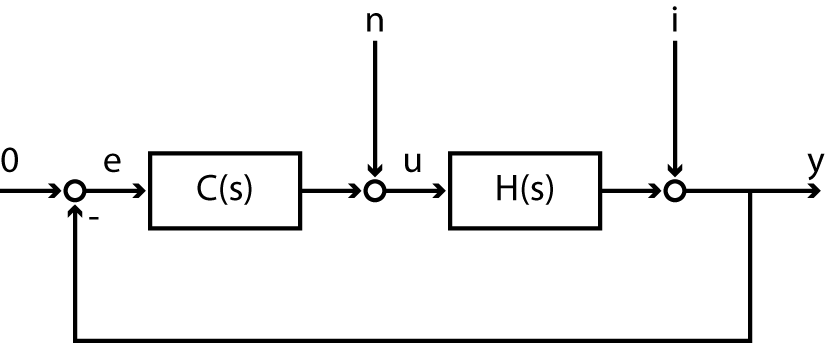
\includegraphics{images/eatonblock}
\end{center}
The system input $e$ and ouput $c$ are measurable and $n$ and $i$ represent unknown sources of noise, which are respectively defined as the remnant and external sources of disturbance.
From the block diagram we can derive that the true transferfunction is defined as:
\begin{align}
		G(s) = \frac{u(s)-n(s)}{e(s)}
\end{align}
Suppose we use the following openloop estimator to identify the transferfunction:
\begin{align}
		\hat{G(s)} = \frac{e^*(s)u(s)}{e^*(s)e(s)}
\end{align}
We get a bias in the estimate, since the noise $n$ is correlated with the error $e$. This correlation occurs because the noise is being fed back to the error. 
\begin{align}
		\hat{G(s)} = G(s) + \frac{e^*(s)n(s)}{e^*(s)e(s)}
\end{align}
However, when we assume a time delay $\tau_G(s)$ in the controller $G$, there exists a short time period where the noise is uncorrelated with the input $e$, so we can write:
\begin{align}
		\frac{e^*(s)n(s)}{e^*(s)e(s)} = 0 \ \ , \ \textrm{for; $\tau \leq \tau_G$}
\end{align}
This fact can be used to remove the bias from the signal, by making use of the physical limiations of the system and using the impulse response method. How they to this exactly remains unclear to me, additional information can be found in Eaton (1973) and in Wingrove and Edwards (1968).
\subsection{Conclusion}
The following citation is taken over from Wingrove and Edwards:
\begin{quote}
		This paper has shown that in measuring pilot describing
		functions, the identification error due to the correlation
		of the input error signal wvith the pilot's output noise can
		be reduced by shifting the input data during the computer
		analysis. The value for this time shift should be near the
		time delay of the pilot. It is shown that this idenitification
		error can be made small if the autocorrelation function
		$R_{nn}(r)$ of the internal noise source is negligible for $r$
		greater than the sum of all transport lags through the
		control loop. This means that if these conditions are met,
		it is possible to measure the describing function of a
		system with feedback, using only its own internal noise
		source for excitation.
\end{quote}
\subsection{Pros and Cons}
\begin{itemize}
		\item[+] No external perturbations required, since the instability of the machine results in a input spectrum. 
		\item[-] There is no control of the input spectrum, because it results from the rider machine interaction. This potentially could result in a limited input spectrum. However the results of Eaton show that it is possible to succesfully estimate the rider action.
		\item[-] Theory is only valid for separete rider machine systems, which are often used within McRuer theory. Unfortuneatly rider control seems to be much more interconnected with the system (multiple feedback loops, different time delays, etc).
		\item[+] The theory would be interesting to apply on the current bicycle simulator, which only makes use of visual feedback.
\end{itemize}
%\citep{wingrove2007measurement}
%\bibliographystyle{plain}
%\bibliography{articles}
 
\chapter{Steer dynamics}
In the Whipple bicycle model, the steering wheel is modeled as a simple frictionless 1DoF rotational joint. In practice the dynamic behavior of this joint is expected to be more complex, for example; viscoses damping may be present due to air damping and Coulomb friction may occur due to friction caused by the bearings. Also some backlash is is observed, which is probably caused by the  torque limiter. The described effects may cause additional steering torques, which are not caused by the rider action. For rider identification, it is important to separate the system dynamics from the rider action. Therefore, the goal of this analysis is to quantify the dynamic properties of the steering joint.
\section{Experiment}
An simple experiment is set up to investigate the dynamic properties of the steering column. 2 springs are attached to the steer to create a known steering torque input, effectively creating a simple spring, mass and damper system. The small angle approximation of the torque caused by the 2 springs is given by:
		\begin{align}
		T_k = 2ek(\delta-\delta_0)
		\end{align}
Where $e$ represents the length of the moment arm, $k$ represents the spring stiffness and $\delta$ represents the angle. The steering angle $\delta$ is measured by using a pod meter. The steering rate is obtained by finite differencing of the steering angle. The rear frame of the bike is fixed to the external world and is assumed not moving at all. The measured parameters of the set up are shown in table \ref{table:measureparms}. Figure \ref{fig:example} shows a typical measurement. Here the steerangle is first set into a unstable position, before it is released at $t=\approx0.8$ [s]. The steer oscilates until it reaches its equilibrium position. 6 Measurements are peformed, consisting of 3 left and 3 right releases. A suitable datarange is selected by making use of the energy aproximation which corresponds to the desired small angle of 0.1 rad in combination with a fixed number of sucseeding datapoints.
\subsection{Calculating spring stiffnes}
The spring stiffness is determined by suspending the spring vertically and measure its length before and after a known amount of mass is added. The following spring stiffness is obtained.
\begin{align}
		k = \frac{\Delta F}{\Delta l} = \frac{g\Delta m}{l_2-l_1} = 912.77 \pm 66 \ \ \textrm{[N/m]}
\end{align}
\subsection{Data selection}
A suitable range of data is chosen based on the estimated energy of the system. The total energy of the system is decreasing because of the dissipation of energy caused by viscous damping and Coulomb friction. When the energy level exceeds a certain tress-hold (corresponding with the potential energy equal to 0.1 rad) the first data point is selected. Secondly, a fixed number of succeeding data-points is selected to complete the datarange. The selection method is shown in figure \ref{fig:energysel} and the resulting dataset for all six measurements is shown in figure \ref{fig:deltasel}. 
		\begin{table}
				\centering
				\begin{tabular}{cccl}
				\toprule
				Symbol & Value & Units & Description \\
				\midrule
				$l_1$ 	& $0.165\pm0.002$ & [m] & spring length 1 \\
				$l_2$ 	& $0.204\pm0.002$ & [m] & spring length 2 \\
				$\Delta m$ 	& $3.628$ & [kg] & added mass \\
				$e$ 		& $0.231\pm0.003$  & [m]	& moment arm \\
				\bottomrule
				\end{tabular}
				\caption{}
				\label{table:measureparms}
		\end{table}		
		\begin{figure}
			\centering
				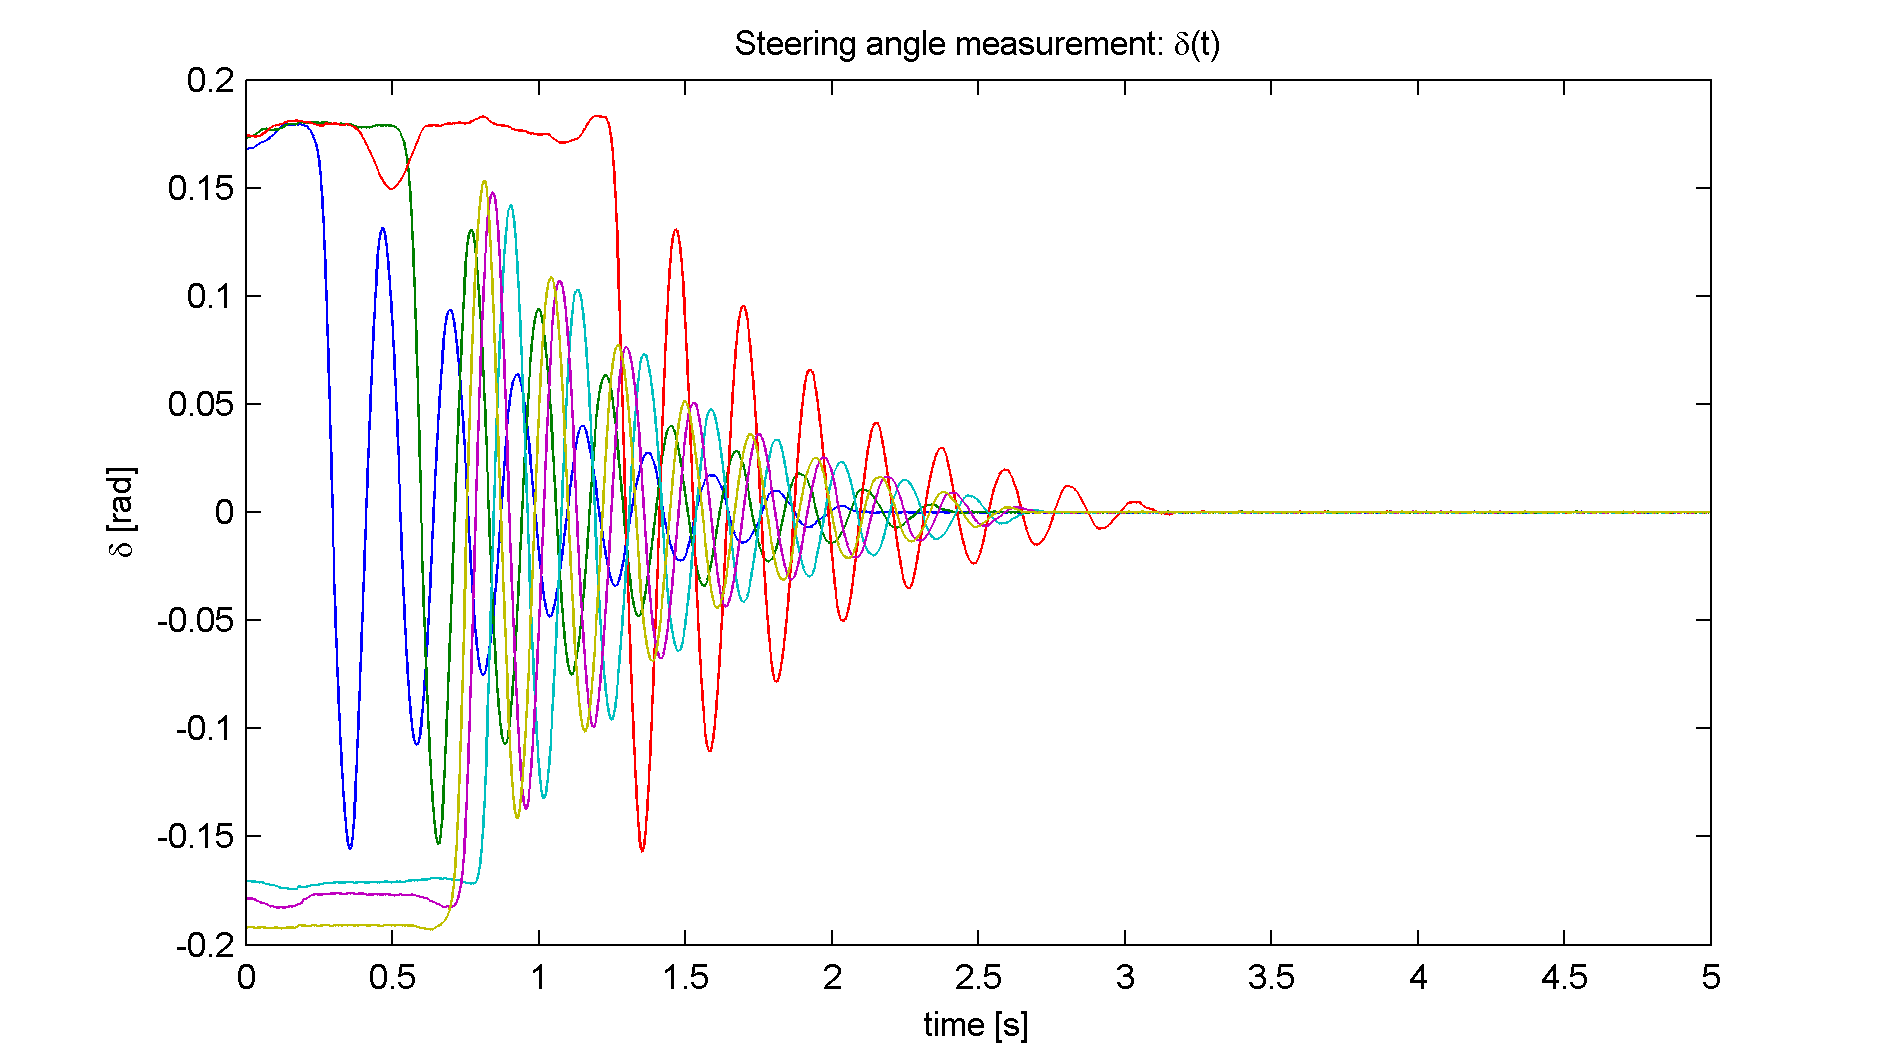
\includegraphics{images/example}
				\caption{}
				\label{fig:example}
		\end{figure}
		\begin{figure}
			\centering
				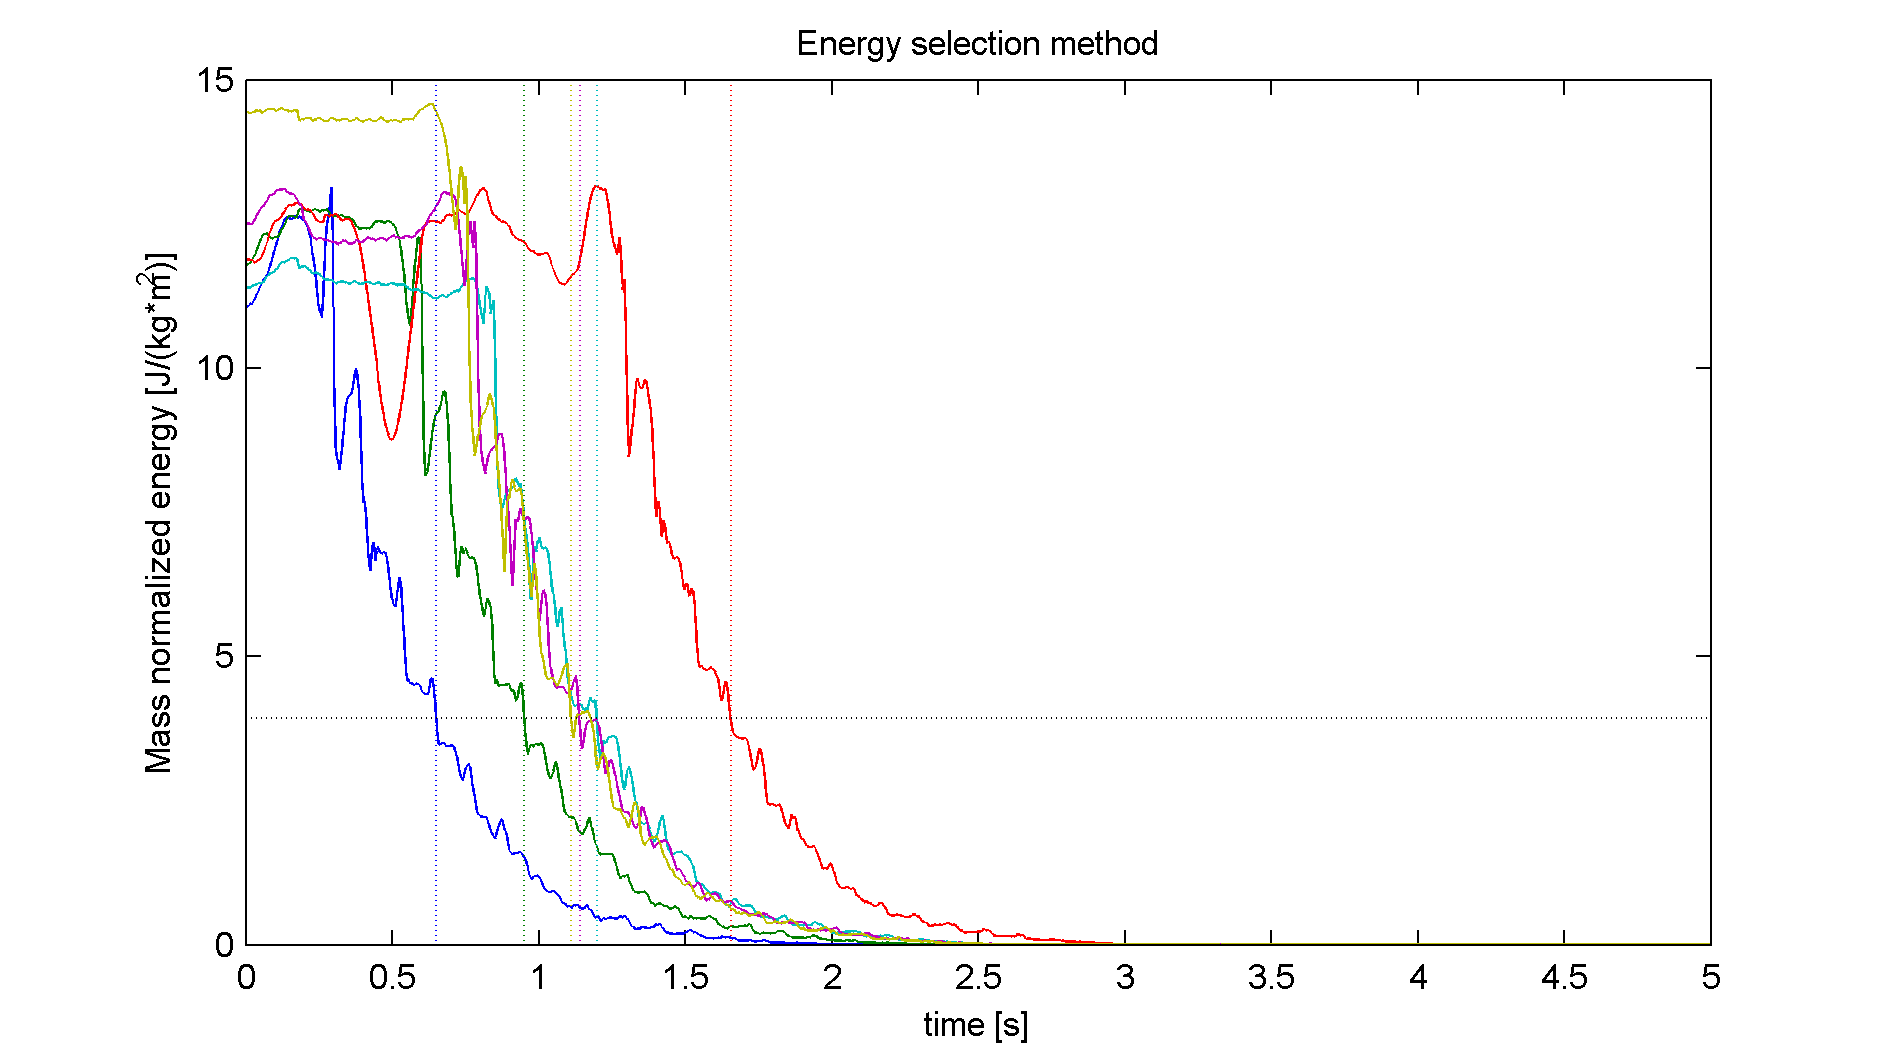
\includegraphics{images/energysel}
				\caption{Datarange selection based on estimated energy. The horizontal line represents the energy tresshold. The vertical lines represent the crossings of the tresshold values, which will be used as the first datapoint. Secondly a fixed range of sucseeding datapoint is selected to complete the selection.}
				\label{fig:energysel}
		\end{figure}
		\begin{figure}
			\centering
				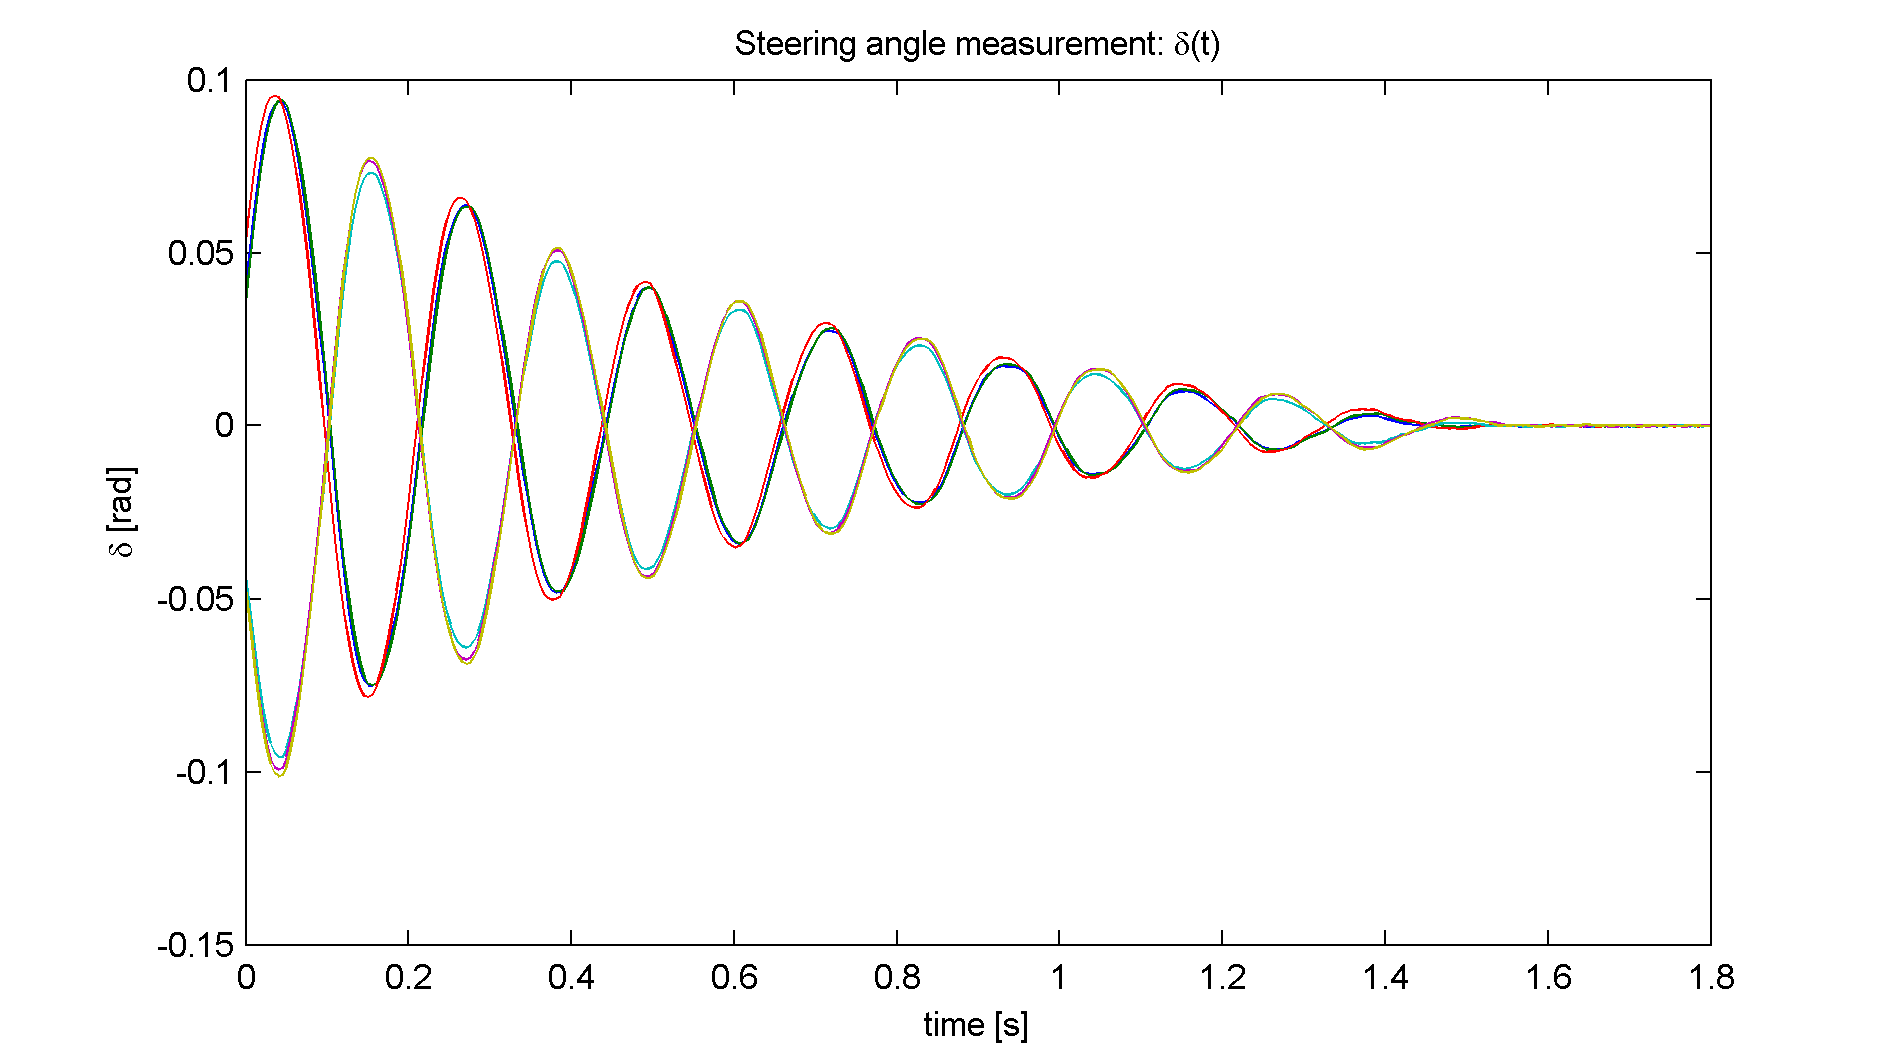
\includegraphics{images/deltasel}
				\caption{Selected datasets}
				\label{fig:deltasel}
		\end{figure}
\section{Model}
The dynamics of the font axis are modeled as a spring/mass/damper system with added Coulomb friction:
		\begin{align}
		\ddot{\delta} + 2\omega_0\zeta\dot{\delta} + \omega_0^2\delta =\tilde{F_c} 
		\end{align}
Where the Coulomb friction $\tilde{F_c} = \frac{F_c}{I_{\delta\delta}}$ is modeled as:
		\begin{align}
		\tilde{F}_c &= \left\{
				\begin{array}{rl}
				 A & \text{if } \dot{\delta} < 0,\\
				0 & \text{if } \dot{\delta} = 0 ,\\
							-A & \text{if } \dot{\delta} > 0.
				\end{array} \right.
		\end{align}
The Coulomb friction introduces an non-linear term in the differential equations. A time series solution of the non linear equations is obtained using the Matlab ODE45 solver. The unknown parameters $\zeta$, $\omega_0$ and $A$ are obtained from the experimental data by using parameter estiamation techniques. Here a Levenberg Marquad algorithm is used for estimating the parameters. 
\section{Results}
The identification algorithm is repeated for 6 measurements. The resulting parameters are shown in the table below: 
%		\begin{table}
				\begin{center} 
				\begin{tabular}{cccc}
				\toprule
				$n$ & $\omega_0$ & $\zeta$ & $A$ \\
				\midrule
				1  & 27.7347  &  0.0455  &  0.9963\\
				2	& 27.7179  &  0.0493  &  0.7559\\
				3	& 27.7228  &  0.0539  &  0.7166\\
				4	& 27.6573  &  0.0505  &  0.7078\\
				5	& 27.5571  &  0.0307  &  1.6129\\
				6	& 27.5462  &  0.0533  &  0.5515\\
				\bottomrule
				\end{tabular}
				\end{center}
The resulting fits are shown in figure \ref{fig:fitting}. Since both the eigenfrequency and stifness are known, a estimate of the mass moment of inertia can be made:
\begin{align}
\omega_0^2 = \frac{2ke}{I_{\delta\delta}}  \ \Rightarrow \  I_{\delta\delta} = \frac{2ke}{\omega_0^2} = 0.55\pm0.04 \ \textrm{[kg/m$^2$]}
\end{align}
%				\caption{}
%				\label{table:parms}
%		\end{table}
		\begin{figure}
			\centering
				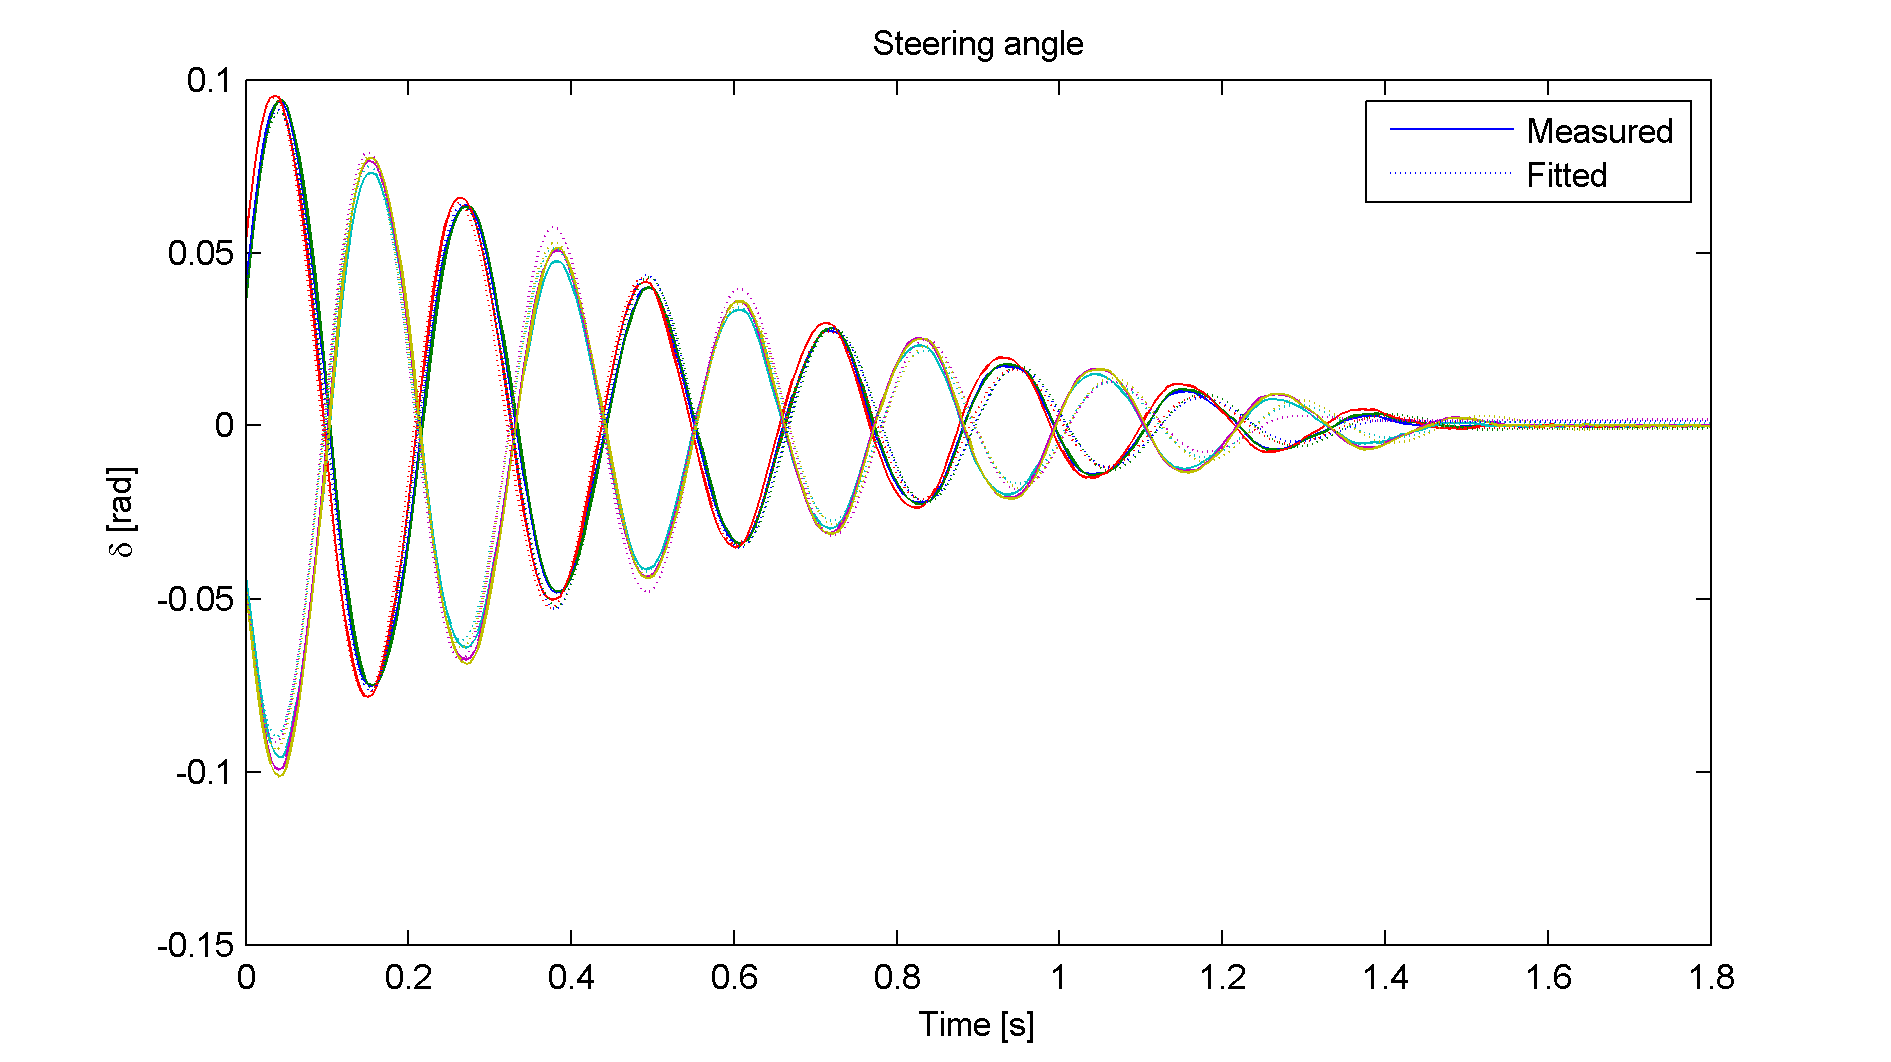
\includegraphics{images/fitting}
				\caption{}
				\label{fig:fitting}
		\end{figure}
\section{Application}
To get an idea of the relative influence of the damping on the steering torque measurements, the damping model is applied to some of the actual measurements. First the damping equations are rewritten to obtain the damping torque $F_d$.
		\begin{align}
		F_d =  {F_c}  -  2\omega_0\zeta I_{\delta\delta} \dot{\delta}
		\end{align}
The damping torque is then plotted together with the measured torque to get an idea of the relative amplitude. The result is shown in figure \ref{fig:torque}
		\begin{figure}
			\centering
				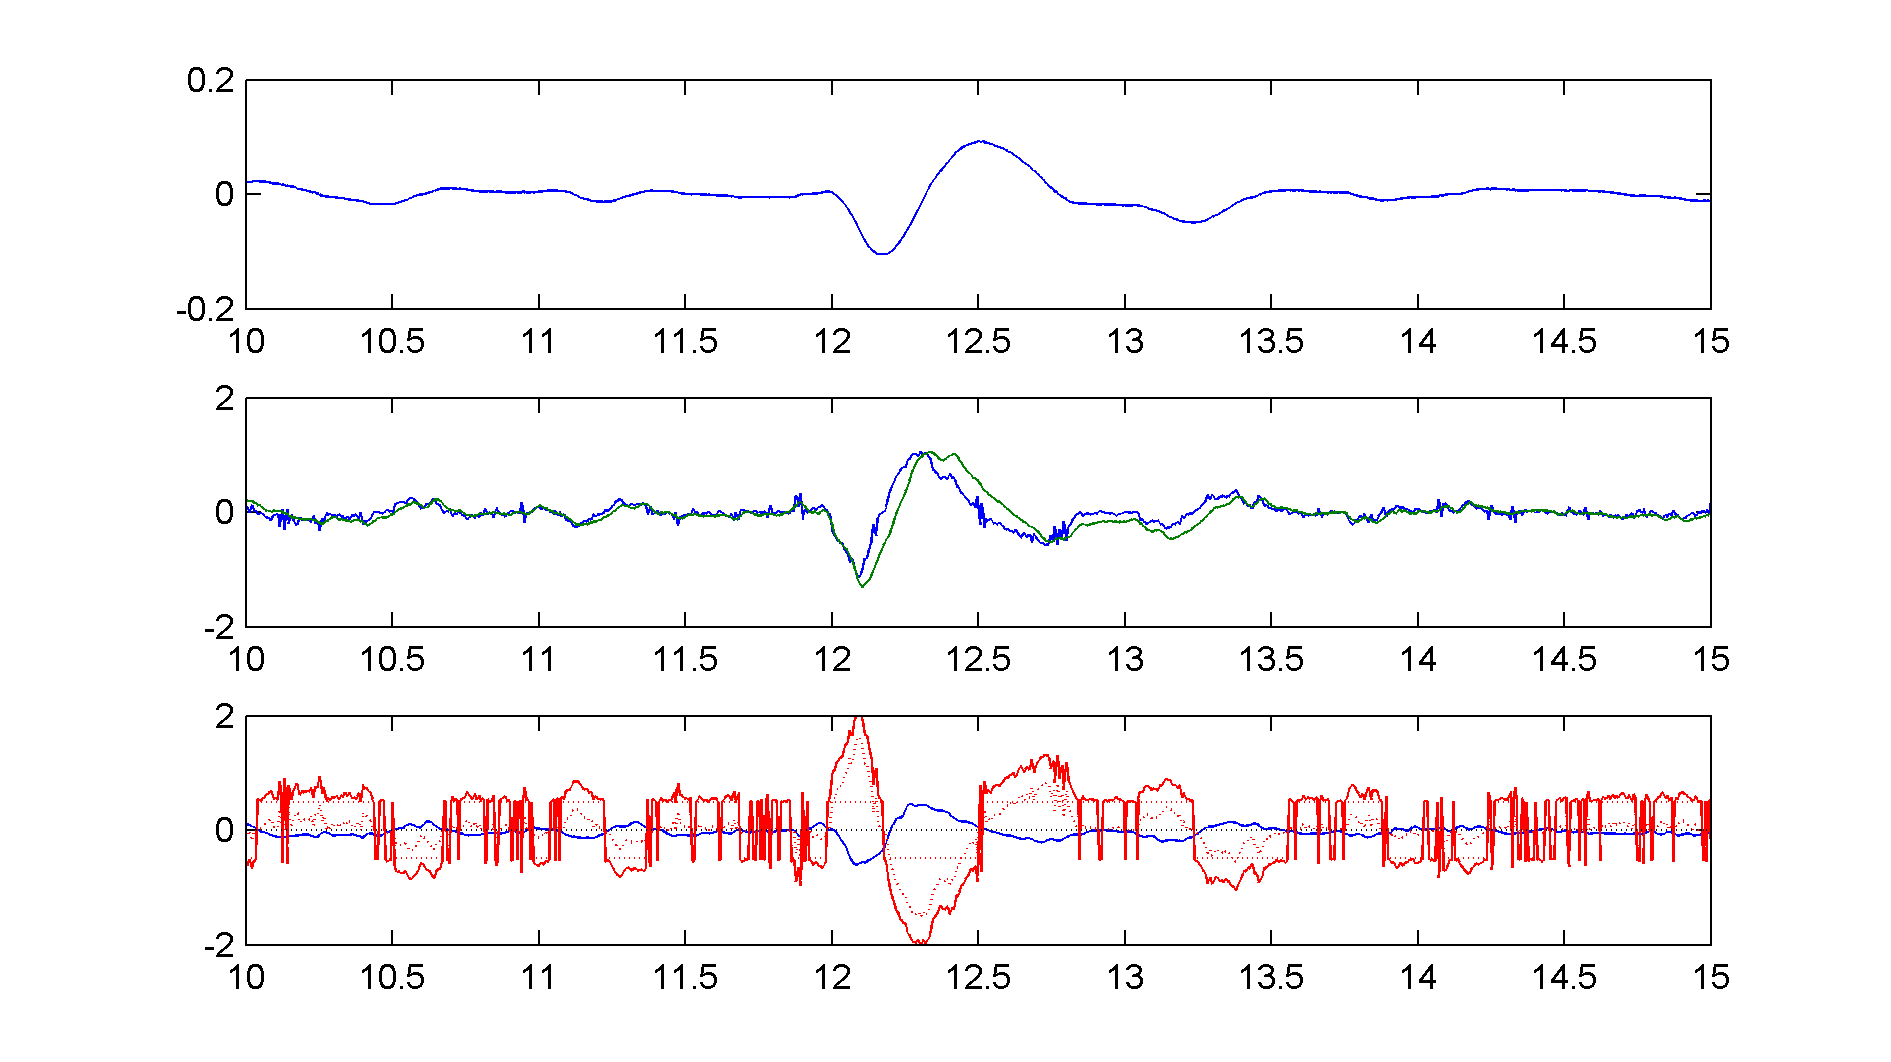
\includegraphics{images/torque}
				\caption{}
				\label{fig:torque}
		\end{figure}
\section{Discussion}
\begin{itemize}
\item Eigenfrequency very consistent
\item Both the Coulomb friction and viscous damping show relatively a lot of variation
\item System seems to be symmetric around $\delta_0$. 
\item Model fits amplitude very well
\item Model has trouble matching the phase.
\end{itemize}
\section{Conclusion}
		\begin{itemize}
				\item Total amount of friction seems to be significant and may not be omitted.
				\item Friction is consists of viscous damping and Coulomb friction.ous damping and Coulomb friction.
		\end{itemize}
\section{Future work} 
		\begin{itemize}
				\item Figure out backlash principle and model it mathematically, incorporate there results in the bike model.
				\item Apply friction model combined with separate inertia models to obtain rider steering torque. 
		\end{itemize}
\section{Some additional analysis}
Figure \ref{fig:steer1} and \ref{fig:steer2} show some additional analysis of the steer dynamics.
		\begin{figure}
			\centering
				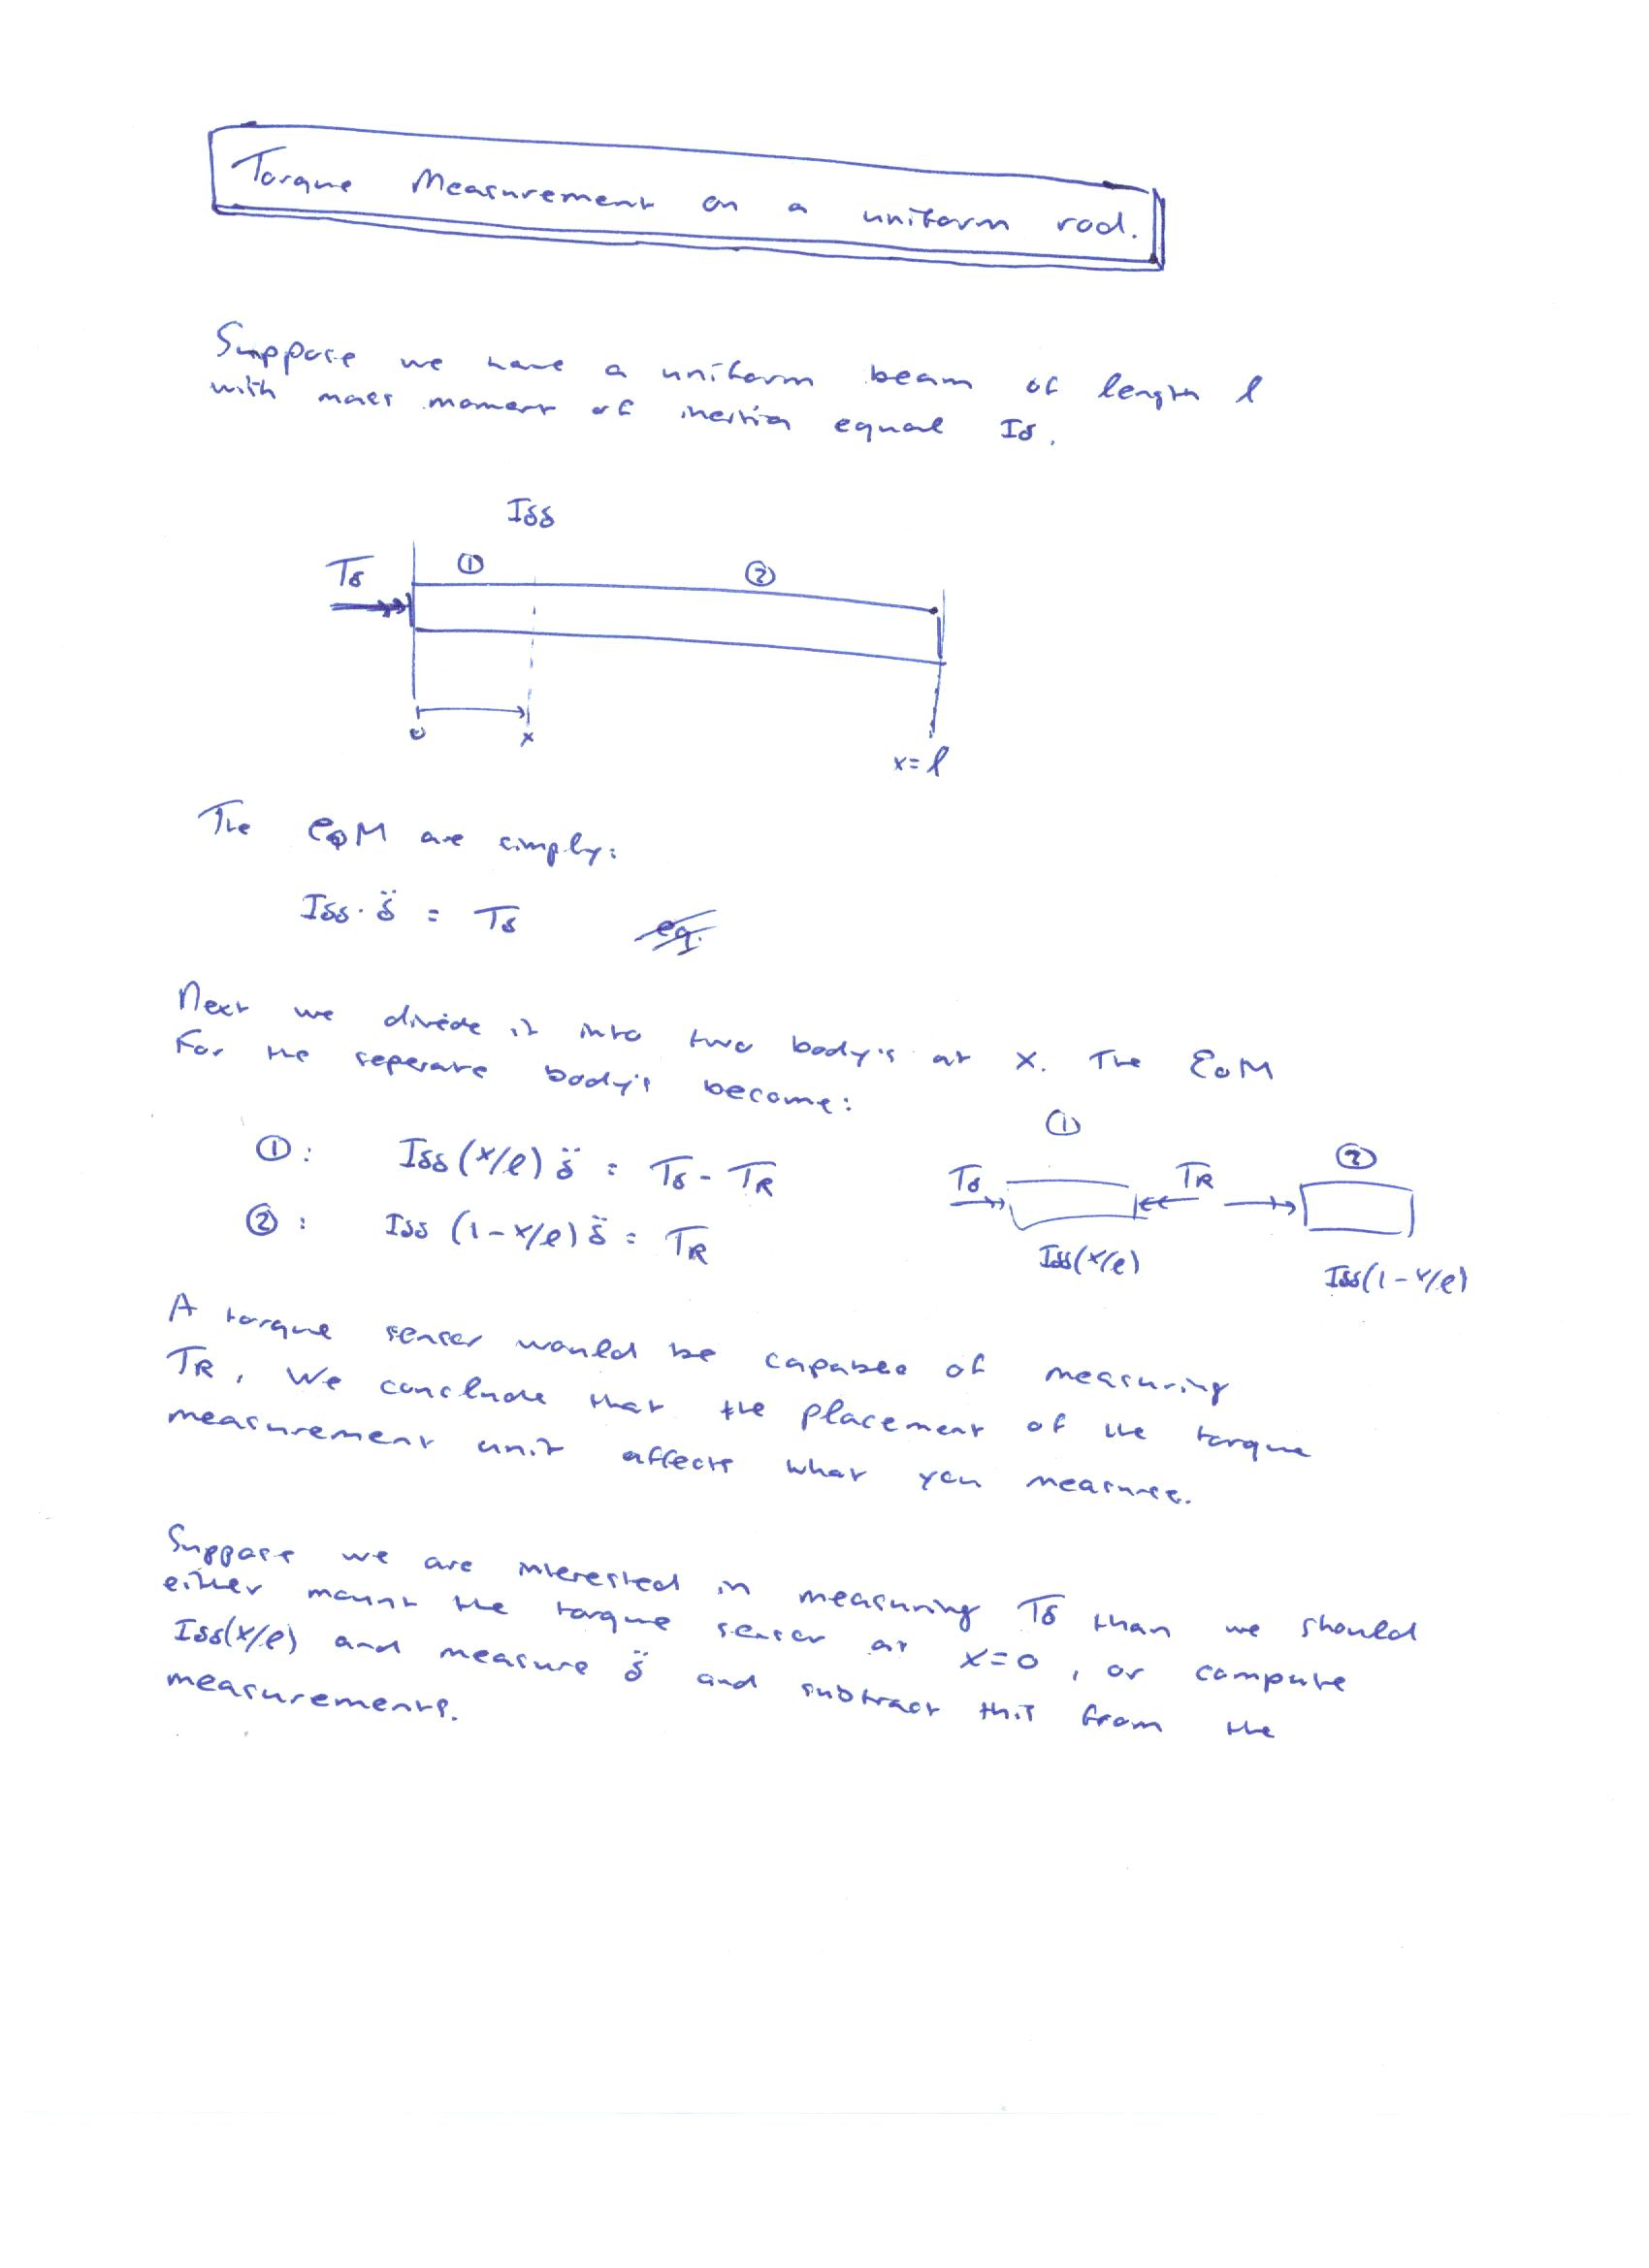
\includegraphics[width=16cm]{images/torquemeasurement.jpg}
				\caption{Torque measurement on uniform bar example}
				\label{fig:steer1}
		\end{figure}
		\begin{figure}
			\centering
				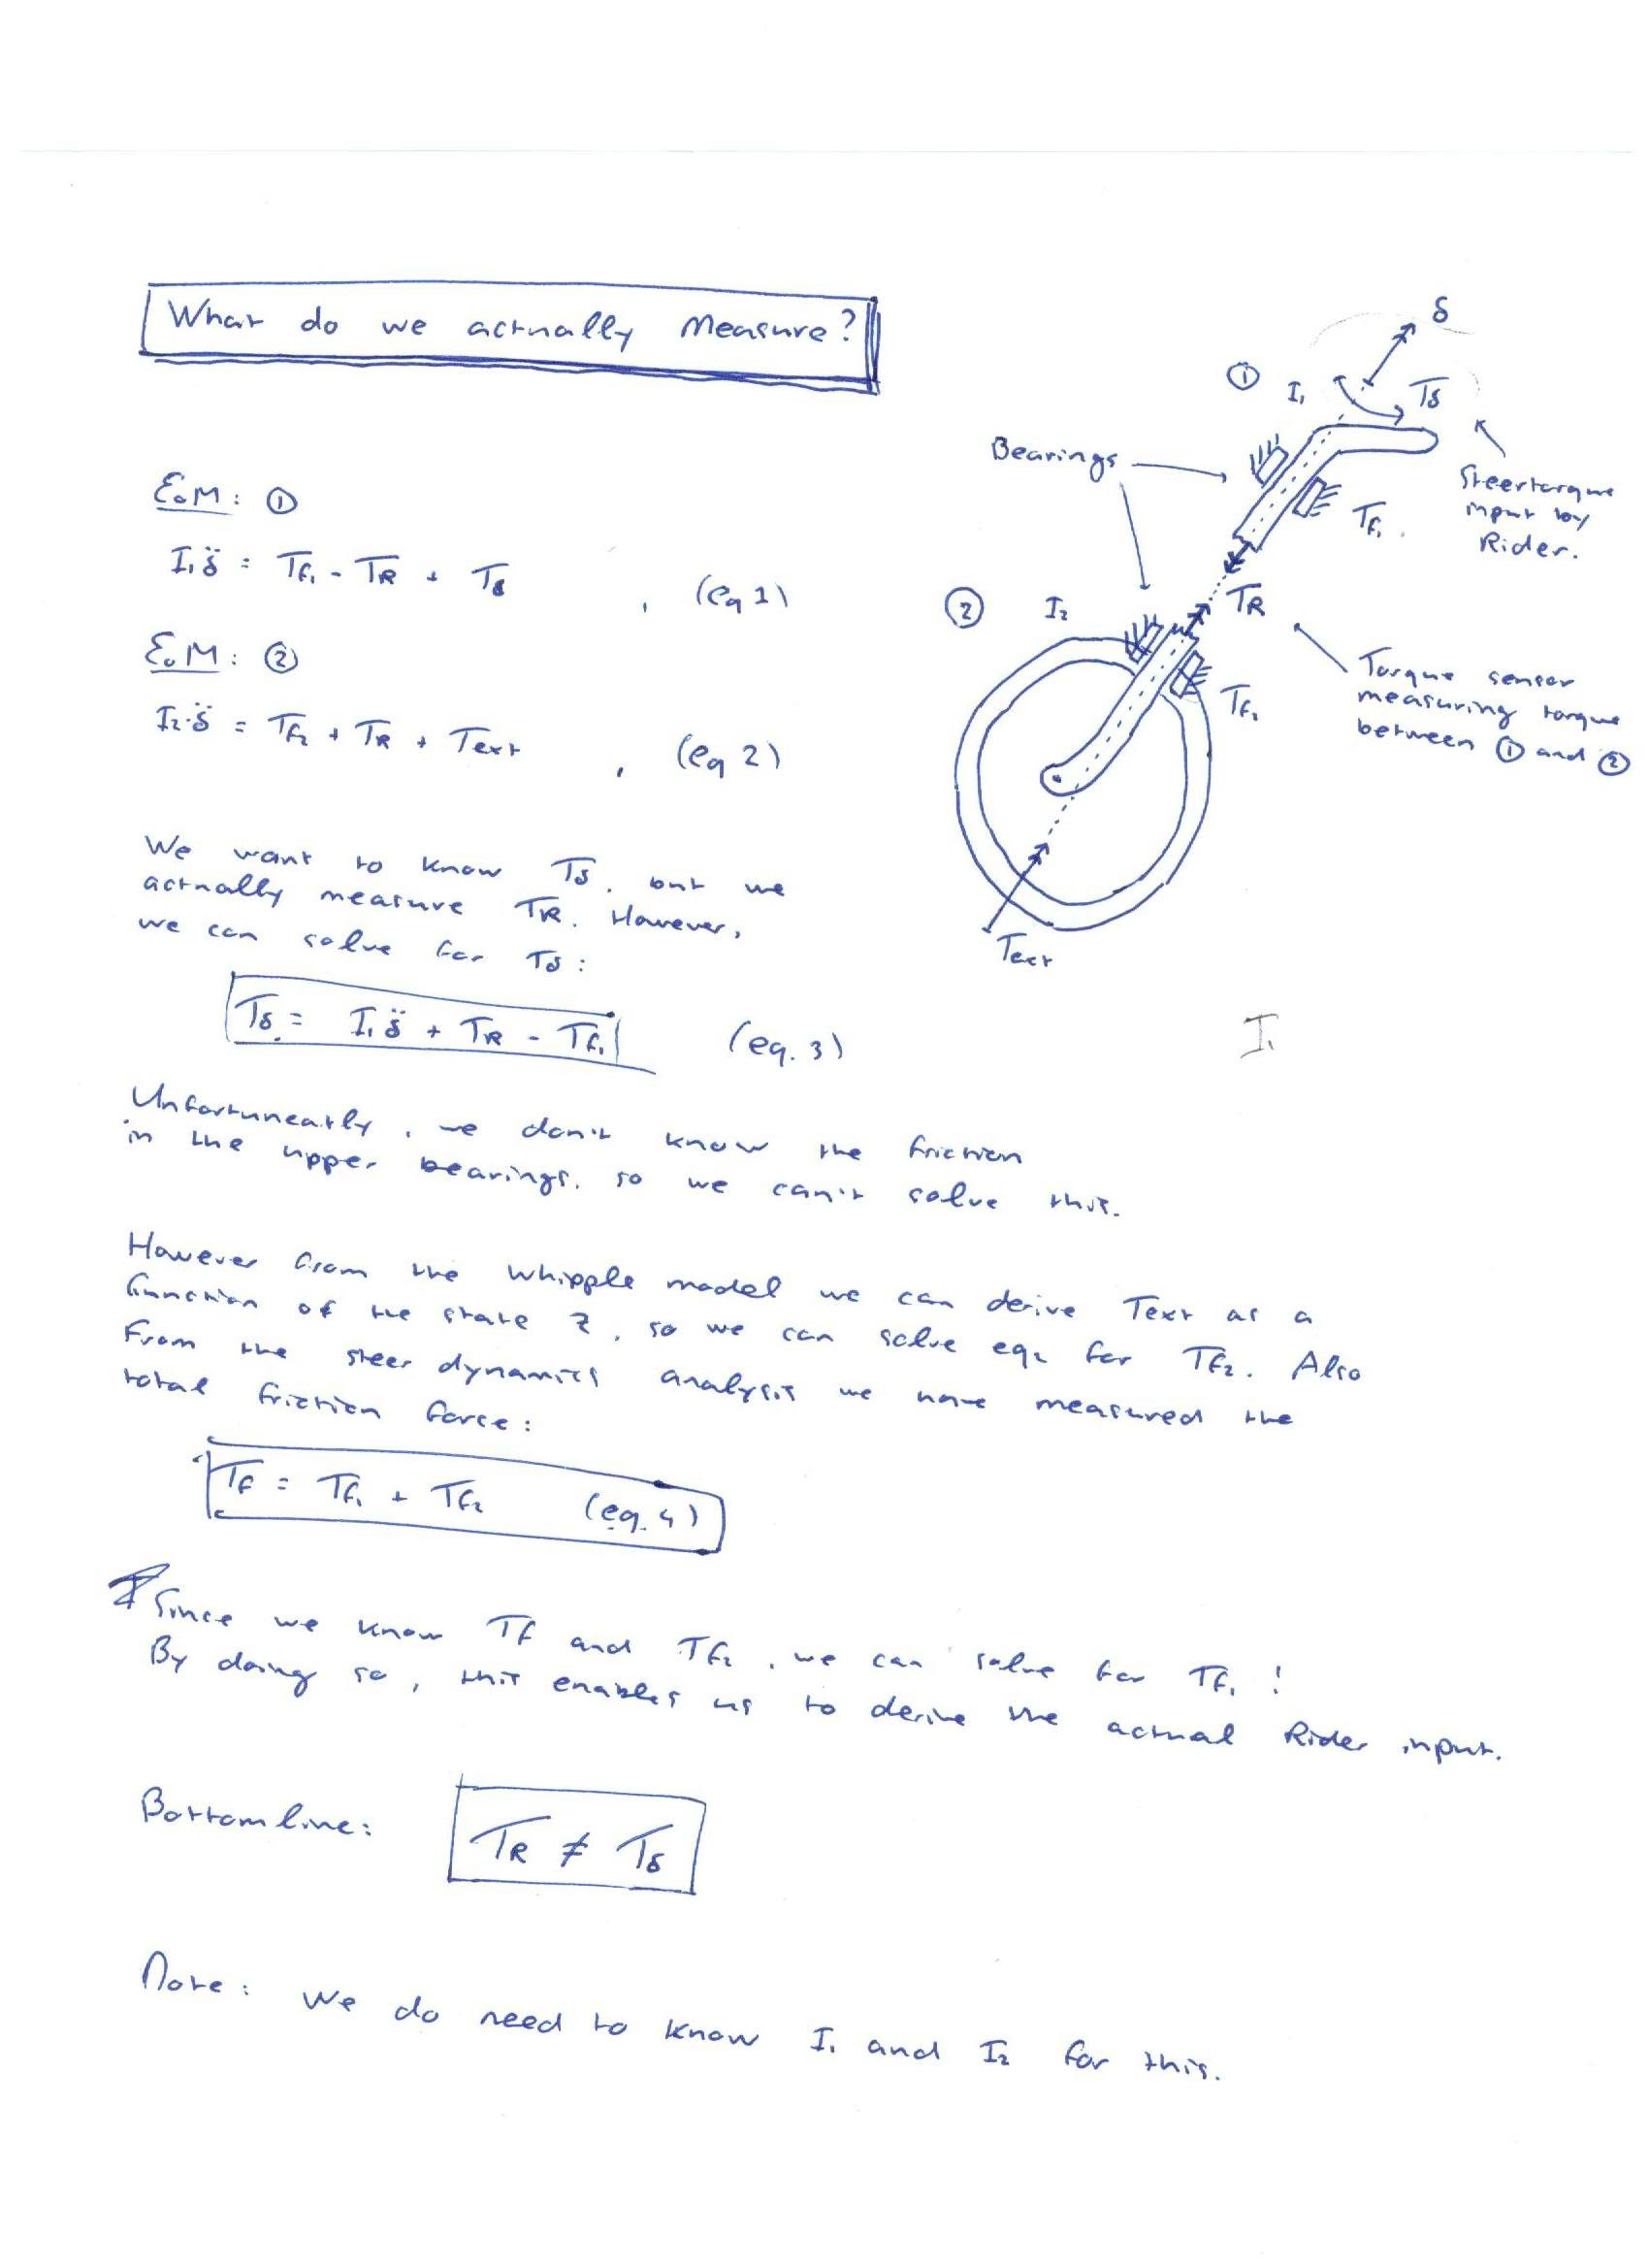
\includegraphics[width=16cm]{images/steeringequations.jpg}
				\caption{Equations of motion governing the steering dynamics}
				\label{fig:steer2}
		\end{figure}
\end{document} 
\end{document}
 